\documentclass[11pt,a4paper]{article}
\usepackage[T1]{fontenc}
\usepackage[utf8]{inputenc}
\usepackage[english]{babel}
\usepackage{geometry}
\geometry{margin=2.5cm}
\usepackage{xcolor}
\usepackage{booktabs}
\usepackage{array}
\usepackage{graphicx}
\usepackage{tikz}
\usetikzlibrary{shapes.geometric,arrows.meta,positioning,fit}
\usepackage{fancyhdr}
\usepackage{hyperref}
\usepackage{listings}
\usepackage{amsmath}
\usepackage{longtable}

\hypersetup{colorlinks=true,linkcolor=blue,urlcolor=blue,citecolor=blue}

\lstset{
  basicstyle=\ttfamily\small,
  breaklines=true,
  frame=single,
  backgroundcolor=\color{gray!8},
  columns=fullflexible,
}

\graphicspath{{figures_campaign2/}}
\setlength{\headheight}{14pt}
\pagestyle{fancy}
\fancyhf{}
\fancyhead[L]{Campaign 2 --- ICOHP Descriptors and Thermodynamic Stability}
\fancyhead[R]{\thepage}
\renewcommand{\headrulewidth}{0.4pt}

\title{\bfseries ICOHP Descriptors and Thermodynamic Stability \\
Across a 349-Structure Dataset \\
\large Campaign 2: Dataset Construction, VASP+LOBSTER Computation,
and Statistical Analysis}
\author{Gilles Frapper \\ Professor, Theoretical Chemistry \\ IC2MP UMR 7285 CNRS, Université de Poitiers \\ \href{mailto:gilles.frapper@univ-poitiers.fr}{gilles.frapper@univ-poitiers.fr}\\[4pt] \small Report generated as part of the \texttt{viability} project}
\date{August 16, 2026}

\begin{document}
\maketitle

\begin{center}
\small\itshape Update, August 16, 2026: this report is reorganized around
the project's current central question --- $\Delta$(ICOHP) and viability
discrimination (\S\ref{sec:reframing}) --- rather than around the
percolation weight, the original campaign 2 subject. Everything
concerning the percolation weight and its direct descendants (network
dimensionality, periodic min-cut --- missions \#1 and \#3) has been moved
to Appendix~\ref{sec:appendix-percolation}, ``Percolation\_viability,''
with the corresponding source code relocated to the repository's
\texttt{Percolation\_viability/} directory. The main body below documents
the project's current state (349 structures, missions \#4--\#5, the
\texttt{extension4} campaign, the $\Delta$(ICOHP) reframing) without
altering the results themselves.
\end{center}

\tableofcontents
\newpage

\section{Objective and Problem Statement}

\textbf{Central research question (see \S\ref{sec:reframing}): does
$\Delta$(ICOHP) --- the reaction-ICOHP descriptor for a compound's
decomposition into elements, and specifically the sign-based
endobondic/exobondic classification it supports --- distinguish
thermodynamically stable, metastable, and unstable compounds?}

This question was built up progressively. The first report (6 toy
compounds) established that a percolation descriptor diverges sharply
from classic ICOHP aggregates, but without a sample large enough to
statistically test whether that difference is \emph{useful}. The
original campaign 2 therefore built a 186-compound dataset to settle
that question --- work whose methodology (dataset selection, statistical
conventions) remains the foundation everything below builds on, but
whose descriptor itself (the percolation weight) and its own result are
now documented in Appendix~\ref{sec:appendix-percolation}, not in this
report's main body: its headline correlation did not survive the
dataset's growth (see \S\ref{sec:followups2}), and it is no longer this
project's organizing question.

Three later missions (network dimensionality/periodic min-cut --- \#3,
also in the appendix; antibonding population --- \#4; reaction ICOHP ---
\#5) and an extension campaign of 163 additional compounds made
$\Delta$(ICOHP) emerge as the project's strongest and most robust
correlation (\S\ref{sec:followups}--\S\ref{sec:followups2}), before the
central question was explicitly reformulated around it
(\S\ref{sec:reframing}).

\section{Methodology}

\subsection{Dataset Selection}

Materials Project query (\texttt{mp\_dataset/select\_campaign.py}) for
the main dataset (186 compounds): unary and binary chemical systems,
non-magnetic ($|\text{total magnetization}| \leq 0.01~\mu_B$/formula
unit --- MP's categorical \texttt{magnetic\_ordering} field is
"Unknown" for $\sim$98\% of entries and would have excluded nearly every
genuinely non-magnetic compound), no f-block elements, $\leq 20$
atoms/cell, 60 compounds per family with a 2-entries-per-chemical-system
cap to ensure elemental diversity rather than many polymorphs of the
same system. Four further extension batches (163 structures,
\S\ref{sec:followups2}) apply the same non-magnetic/no-f filter but with
their own per-mission selection logic (elemental references,
high-pressure polymorphs, alkali/alkaline-earth binaries) --- detailed
in their respective sections, not repeated here.

\subsection{Bonding-Type Classification}

Bond type (ionic / covalent / metallic) is computed by
\texttt{fetch\_candidates.py}'s \texttt{classify()} function
(\textbf{reused unchanged}), from \texttt{is\_metal} and elemental
composition. \textbf{This classification is purely informative in this
report}: a descriptive lens on the dataset (\S\ref{sec:dataset}), not a
sampling axis or a variable any main-body conclusion depends on --- other
mission reports (\texttt{REPORT\_antibonding.md},
\texttt{REPORT\_reaction\_icohp.md}) actively use it to stratify their
own correlations, but that is not its role here.

\subsection{VASP + LOBSTER Computation}

Same template across all 349 structures (static run, \texttt{ISYM=$-1$},
\texttt{LASPH=.TRUE.}, PAW-PBE potentials recommended by
\texttt{pymatgen.io.vasp.sets.MPRelaxSet}): \texttt{NBANDS} is derived
per compound from the number of local orbitals in the LOBSTER basis
(\texttt{Lobsterin.write\_INCAR}), and basis-function determination goes
through \texttt{Lobsterin.get\_basis(potcar\_symbols=\ldots)} rather than
direct POTCAR-file parsing (whose internal pymatgen validity check fails
on several POTCARs unrecognized by hash in the local mirror).

\subsection{Statistics}

Spearman correlation (no reason to expect a linear relationship) between
each ICOHP/ICOBI descriptor and a stability target
(\texttt{energy\_above\_hull} or \texttt{formation\_energy\_per\_atom}
depending on the mission), overall and per subgroup (\texttt{bond\_type},
\texttt{is\_metal}, or selection provenance as appropriate); any $n<15$
subgroup is explicitly flagged, never presented bare. \textbf{No SISSO,
no symbolic regression} at this stage (see
\S\ref{sec:limits-current}).

\section{Workflow Diagram}

\begin{center}
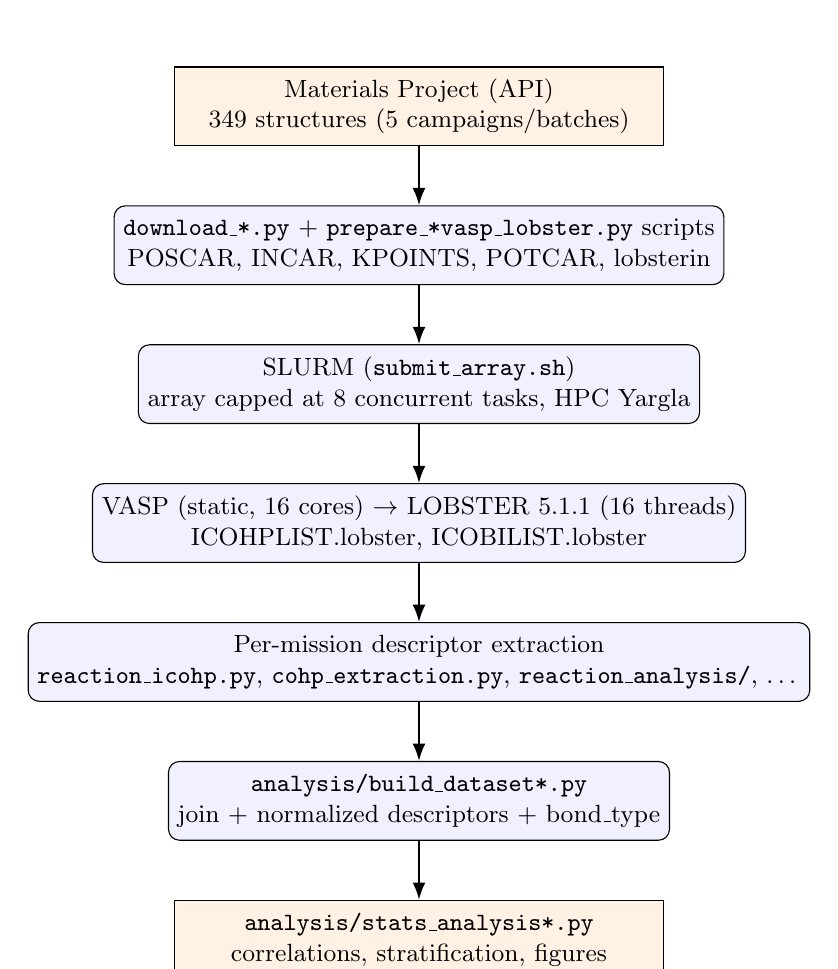
\begin{tikzpicture}[
  node distance=0.75cm and 1.6cm,
  box/.style={draw, rounded corners, minimum width=6.2cm, minimum height=1.0cm,
              align=center, fill=blue!6, font=\small},
  io/.style={draw, minimum width=6.2cm, minimum height=1.0cm, align=center,
             fill=orange!10, font=\small},
  arr/.style={-{Latex[length=2.2mm]}, thick}
]
\node[io]  (mp)     {Materials Project (API) \\ 349 structures (5 campaigns/batches)};
\node[box, below=of mp] (prep)   {\texttt{download\_*.py} + \texttt{prepare\_*vasp\_lobster.py} scripts \\ POSCAR, INCAR, KPOINTS, POTCAR, lobsterin};
\node[box, below=of prep] (slurm)  {SLURM (\texttt{submit\_array.sh}) \\ array capped at 8 concurrent tasks, HPC Yargla};
\node[box, below=of slurm] (vasplob) {VASP (static, 16 cores) $\rightarrow$ LOBSTER 5.1.1 (16 threads) \\ ICOHPLIST.lobster, ICOBILIST.lobster};
\node[box, below=of vasplob] (desc)   {Per-mission descriptor extraction \\ \texttt{reaction\_icohp.py}, \texttt{cohp\_extraction.py}, \texttt{reaction\_analysis/}, \ldots};
\node[box, below=of desc] (join)   {\texttt{analysis/build\_dataset*.py} \\ join + normalized descriptors + bond\_type};
\node[io, below=of join] (stats)  {\texttt{analysis/stats\_analysis*.py} \\ correlations, stratification, figures};

\draw[arr] (mp) -- (prep);
\draw[arr] (prep) -- (slurm);
\draw[arr] (slurm) -- (vasplob);
\draw[arr] (vasplob) -- (desc);
\draw[arr] (desc) -- (join);
\draw[arr] (join) -- (stats);
\end{tikzpicture}
\end{center}

The percolation weight (\texttt{Percolation\_viability/percolation\_path.py})
and its direct descendants (dimensionality, min-cut) follow the same
pipeline upstream of the "descriptor extraction" step but no longer
appear in this diagram, or as this report's subject --- see the original
workflow diagram and the detail of their own processing in
Appendix~\ref{sec:appendix-percolation}.

\section{Environment}

Identical across all 349 structures (Yargla, VASP 6.5.0, LOBSTER 5.1.1,
Python 3.11 \texttt{.venv}), extended with: \texttt{mp-api},
\texttt{pandas}, \texttt{scipy}, \texttt{scikit-learn},
\texttt{matplotlib}, \texttt{pydantic}, \texttt{pyyaml} (see
\texttt{requirements.txt}). Per-step core allocation: \S\ref{sec:cost}.

\section{Dataset}
\label{sec:dataset}

\begin{center}
\begin{tabular}{@{}lrl@{}}
\toprule
Family & $n$ & $E_\text{hull}$ range (eV/atom) \\
\midrule
exp\_stable       & 63  & 0.0000 (by construction) \\
exp\_metastable   & 63  & 0.0005 -- 0.0907 \\
theo\_metastable  & 60  & 0.0013 -- 0.1991 \\
extension (4 batches)$^\dagger$ & 163 & heterogeneous, see \S\ref{sec:followups}--\S\ref{sec:followups2} \\
\midrule
\textbf{Total}    & \textbf{349} & \\
\bottomrule
\end{tabular}

\vspace{0.15cm}
{\footnotesize $^\dagger$ elemental references, TiO$_2$/carbon
high-pressure polymorphs, and alkali/alkaline-earth binaries
(\texttt{extension4}) --- full composition in
Appendix~\ref{sec:appendix-ext-elements}--\ref{sec:appendix-ext-compounds}.}

\vspace{0.3cm}

\begin{tabular}{@{}lr@{}}
\toprule
Composition & $n$ \\
\midrule
Single-element references & 68 \\
Multi-element compounds   & 281 \\
\midrule
\textbf{Total}             & \textbf{349} \\
\bottomrule
\end{tabular}

\vspace{0.3cm}

\begin{tabular}{@{}lr@{}}
\toprule
Bond type (\texttt{classify()}, informative only) & $n$ \\
\midrule
metallic       & 88 \\
ionic          & 53 \\
covalent       & 35 \\
unclassified   & 173 \\
\midrule
\textbf{Total}  & \textbf{349} \\
\bottomrule
\end{tabular}
\end{center}

The "bond type" table was \textbf{not out of date by accident}: the
\texttt{extension4} campaign (\S\ref{sec:followups2}) specifically added
89 alkali/alkaline-earth binaries against N/O/F/P/S/Cl, taking the ionic
total from 9 (campaign 2 alone) to 53. Half of these new binaries
nonetheless remain "unclassified": \texttt{classify()} only recognizes
alkali/alkaline-earth $\times$ \{halogen, O\} pairs as "ionic"
(\texttt{IONIC\_ANIONS}), not $\times$ \{N, P, S\} --- a real limitation
of the reused heuristic, documented but not fixed here. As noted in
\S2.2, this categorization remains purely descriptive in this report.

\section{Results}
\label{sec:results}

\subsection{Correlations (Spearman) --- classic ICOHP aggregates}

\begin{center}
\small
\begin{tabular}{@{}llrrr@{}}
\toprule
Group & Metric & $n$ & $\rho$ & $p$ \\
\midrule
all & ICOHP sum    & 186 & 0.032 & 0.670 \\
all & ICOHP min    & 186 & 0.093 & 0.209 \\
metallic & ICOHP sum  & 88 & 0.223 & 0.037 \\
metallic & ICOHP min  & 88 & 0.198 & 0.065 \\
\bottomrule
\end{tabular}
\end{center}

These four rows (classic ICOHP aggregates, campaign 2, $n=186$, target
\texttt{energy\_above\_hull}) are kept here as the reference baseline
for every later mission. \textbf{The percolation weight, which appeared
in this same table in the original version of this report, is moved in
full to Appendix~\ref{sec:appendix-percolation}} (complete table with
bond-type subgroups, reference logistic regression, and associated
figures) --- this trimmed table therefore no longer allows a direct
percolation-vs-classic-aggregates comparison; that comparison is still
available as-is in the appendix. Current descriptors' correlations
(antibonding population, reaction ICOHP) are given in
\S\ref{sec:followups}--\S\ref{sec:followups2}, against
\texttt{formation\_energy\_per\_atom} rather than
\texttt{energy\_above\_hull}.

\section{Failures Found and Fixed}

Per the instruction ("every job failure must be logged with its probable
cause"), 5 of the 178 SLURM-array-submitted jobs failed on the first
pass while computing campaign 2's 186 compounds, all diagnosed and fixed
at the source (the fixes, applied to the shared SLURM/INCAR templates,
carry over to every later campaign):

\begin{itemize}
  \item \textbf{Al12W, BW, WO2, TcW, TiW} (all tungsten-containing): the
    local mirror's \texttt{W\_sv} POTCAR is missing its \texttt{LEXCH}
    field entirely (confirmed by direct inspection --- present in every
    other variant checked, including plain \texttt{W}), which VASP reads
    as an incompatible exchange-correlation functional and refuses to run.
    Fixed by replacing the \texttt{W\_sv} override with plain \texttt{W}
    (valid PBE, verified).
  \item \textbf{Al12W} failed again after that fix, this time with a VASP
    SIGSEGV --- exactly the known issue flagged in the mission brief
    (\texttt{ulimit -s unlimited} before \texttt{vasp\_std}), present in
    \texttt{submit\_array.sh} but forgotten in
    \texttt{prepare\_vasp\_lobster.py}'s per-compound SLURM template.
    Fixed; recovered on retry.
\end{itemize}

Final success rate across all 349 structures computed to date:
\textbf{349/349}.

\section{Compute Cost}
\label{sec:cost}

\textbf{349 structures computed in total}: 68 single-element references
and 281 multi-element compounds (\S\ref{sec:dataset}), across five
submission campaigns/batches (the original campaign 2 and four
\texttt{extension} batches).

Every VASP job, then LOBSTER job, runs on the \textbf{Yargla} HPC cluster,
within a single SLURM allocation of one node (\texttt{--nodes=1}) and
\textbf{16 cores}: VASP under MPI parallelism
(\texttt{--ntasks=16 --cpus-per-task=1}, \texttt{srun}), then LOBSTER
under OpenMP parallelism on the same 16 cores
(\texttt{OMP\_NUM\_THREADS=16}, single process, run sequentially after
VASP within the same job). The SLURM array (\texttt{submit\_array.sh}) is
capped at 8 concurrent tasks.

\begin{center}
\begin{tabular}{@{}lrr@{}}
\toprule
 & VASP & LOBSTER \\
\midrule
$n$ & 349 & 348$^*$ \\
Mean (s) & 168 & 404 \\
Median (s) & 58 & 110 \\
Max (s) & 5715 (1.6 h) & 12063 (3.4 h) \\
Sequential total & 16.3 h & 39.0 h \\
\bottomrule
\end{tabular}

\vspace{0.15cm}
{\footnotesize $^*$ 1 of 349 structures had no usable LOBSTER step
(trivial-cell reference element).}
\end{center}

Combined sequential total (VASP + LOBSTER, 349 structures):
\textbf{55.3 h}. Given the 8-concurrent-task cap, the order of magnitude
for actual elapsed time to process this volume as a single batch would
be $\sim$6.9~h --- a rough estimate (dividing by 8, ignoring queue time)
given for context: in practice, the 349 structures were submitted across
several campaigns spread over multiple sessions, not as one single
batch.

\section{Current Limits and Next Steps}
\label{sec:limits-current}

\begin{itemize}
  \item \textbf{\texttt{classify()} coverage}: 173/349 structures (50\%)
    fall outside the ionic/covalent/metallic categories, mostly
    alkali/alkaline-earth $\times$ \{N, P, S\} bonds that
    \texttt{IONIC\_ANIONS} does not recognize (\S\ref{sec:dataset}) ---
    purely informative here, but a real limitation for any mission that
    would want to stratify on it.
  \item \textbf{No true dynamical "unstable" class}: \texttt{theo\_metastable}
    and the theoretical \texttt{extension} batches are proxies (never
    synthesized), not a phonon-calculation result.
  \item \textbf{Per-subgroup sample size}: remains this project's
    structural limit at every new stratification (\texttt{bond\_type},
    \texttt{is\_metal}, \texttt{family}) --- see
    \S\ref{sec:followups}--\S\ref{sec:followups2} for concrete examples
    where an $n<15$ subgroup did not replicate once the sample grew.
  \item \textbf{Why not SISSO yet}: reaction ICOHP (mission \#5,
    \S\ref{sec:followups2}) is now the strongest correlate and the first
    whose signal is not fully explained away by between-group clustering
    at every level tested --- the best argument yet for a stratified
    feature search, still not attempted.
\end{itemize}

Limits specific to the percolation weight and its descendants
(primitive-vs-conventional-cell sensitivity, chance-level reference
logistic regression) are documented in
Appendix~\ref{sec:appendix-percolation}, not repeated here.

\section{Conclusion}

The dataset grew from 186 to 349 computed structures (VASP+LOBSTER)
across five campaigns/batches, with a final success rate of 349/349 and
two compute failures diagnosed and fixed at the source during the
original campaign 2. The project's organizing question evolved along the
way: starting from the percolation weight (no significant correlation
retained, Appendix~\ref{sec:appendix-percolation}), through network
dimensionality/periodic min-cut (also in the appendix, headline
correlation not reproduced at the current scale), the antibonding
population near the Fermi level (mission \#4, the project's most robust
covalent subgroup), to reaction ICOHP and its endobondic/exobondic
classification (mission \#5) --- now the project's strongest and most
robust correlation, and the central question explicitly reformulated
around it (\S\ref{sec:reframing}). The next concrete milestone, already
identified in the reframing, is a deliberate extension to compounds near
the stability edge rather than continuing to accumulate compounds that
are comfortably stable or comfortably unstable.

\vspace{1cm}
\noindent\textit{Source code:} \url{https://github.com/John-Akapulco/viability} \\
\noindent\textit{Data:} \texttt{analysis/percolation\_vs\_formation\_energy.csv} \\
\noindent\textit{Detailed reports:} \texttt{analysis/REPORT\_*.md}

\section{Campaign 2 follow-ups (missions \#4 and \#5)}
\label{sec:followups}

Two further descriptors were built in later sessions, both tested
against \texttt{formation\_energy\_per\_atom} (introduced in mission
\#3 as an alternative target to \texttt{energy\_above\_hull}, generally
more correlatable) rather than the hull. Both reuse the 186-compound
dataset above unmodified at the initial stage; mission \#5 draws in part
on a \textbf{74-compound extension campaign} (\texttt{extension\_*}:
elemental references, ionic compounds and polymorphs outside the main
set), detailed in \S\ref{sec:followups2}. Numbers in this subsection are
as of August 15, 2026, at the 186/192-compound scale;
\S\ref{sec:followups2} reprocesses both missions at the 349-compound
scale reached the following day and should be read alongside this
subsection, not instead of it.

\textbf{A pattern repeats across both missions}: each new descriptor
reaches a statistically significant \emph{global} correlation, stronger
than anything the percolation weight or the min-cut ever achieved
(Appendix~\ref{sec:appendix-percolation}) --- but in both cases that
global correlation turns out to be substantially, or entirely, a
clustering effect between bond types or between metals and gapped
compounds, rather than a robust relationship \emph{within} a homogeneous
group.

\subsection{Mission \#4: antibonding population near the Fermi level}

A distinct question from integrated ICOHP (one number per bond): not
\emph{how much} bonding a compound has, but \emph{how} COHP is
distributed in energy --- the occupied antibonding fraction just below
the Fermi level/VBM, by analogy with Peierls/Jahn--Teller electronic
instabilities (new module \texttt{cohp\_extraction.py}, validated by
exact cross-check against \texttt{ICOHPLIST.lobster} on the 6 pilot
compounds). Headline: $\rho=-0.328$, $p=5.0\times10^{-6}$ ($n=186$) ---
the strongest global correlation in the project at the time. The sign is
\emph{opposite} the naive Peierls/Jahn--Teller reading. Diagnostics: the
effect is substantially driven by metal/gapped clustering, but the
\texttt{bond\_type=covalent} subgroup ($n=23$) survives stratification
($p=0.018$--$0.029$) --- the only subgroup in the project, to date, to
hold up under such a test.

\subsection{Mission \#5: reaction ICOHP}

An ICOHP analog of \texttt{formation\_energy\_per\_atom}: is a
compound's total ICOHP "cheaper" than the same atoms in elemental
reference form (new module \texttt{reaction\_icohp.py}, reaction
balanced via \texttt{pymatgen.analysis.reaction\_calculator})? Extended
to 192 compounds using the 74-compound extension campaign (62 elemental
references computed). Headline: $\rho=0.370$, $p=3.9\times10^{-7}$
($n=177$) --- numerically the strongest global correlation in the
project to date, this time with an intuitive sign (less bonding than the
elemental state $\Rightarrow$ less stable formation). But \textbf{no
\texttt{bond\_type} subgroup survives stratification} (Kruskal--Wallis
$p=2.1\times10^{-6}$ for the descriptor, $p=5.0\times10^{-8}$ for the
target, across the three strata) --- unlike mission \#4, the clustering
effect here explains the entire observed signal. Against
\texttt{energy\_above\_hull} the correlation is absent ($\rho=0.09$,
$p=0.20$).

\subsection{Comparison (missions \#4--\#5, 186/192-compound scale)}

On the same common subsample ($n=177$, the intersection of campaign 2's
186 compounds and mission \#5's 192 computable rows):

\begin{center}
\begin{tabular}{@{}lrrr@{}}
\toprule
Descriptor & $n$ & $\rho$ & $p$ \\
\midrule
Reaction ICOHP (mission \#5) & 177 & 0.370 & $3.9\times10^{-7}$ \\
Antibonding population, normalized (mission \#4) & 177 & $-0.337$ & $4.5\times10^{-6}$ \\
\bottomrule
\end{tabular}

\vspace{0.15cm}
{\footnotesize Periodic min-cut (mission \#3, $\rho=0.313$) and
percolation weight (mission \#1, $\rho=0.104$), on the same $n=177$, are
given for reference in Appendix~\ref{sec:appendix-percolation}.}
\end{center}

Ranking by raw correlation strength ($\rho$) is not the same as ranking
by reliability: mission \#5 leads numerically but is also the only one
where \emph{no} subgroup survives stratification, whereas mission \#4
keeps a significant covalent subgroup.

\section{August 16 Update: the extension4 Campaign and Missions \#4--\#5 Reprocessed}
\label{sec:followups2}

\subsection{The extension4 campaign}

89 new compounds (\texttt{mp\_dataset/download\_extension4.py}): binary
compounds of an alkali (Li/Na/K/Rb/Cs) or alkaline-earth (Be/Mg/Ca/Sr/Ba)
metal against N/O/F/P/S/Cl, sourced from Materials Project. Up to 2
compounds picked per (cation, anion) chemical system across 44 systems: an
experimentally-known polymorph (preferring formulas already elsewhere in
the dataset, to build genuine same-composition polymorph groups --- the
dataset had only 8 such groups before this batch) and the
highest-\texttt{energy\_above\_hull} theoretical entry available for that
formula, a deliberate far-from-equilibrium stress test. Selection was
computed once and frozen to \texttt{extension4\_candidates.json} for
reproducibility (scale made hand-curation, the convention for every
earlier extension batch, impractical). All 89 VASP+LOBSTER jobs completed
unattended (a self-healing watcher restarted any job that left the SLURM
queue without producing output; zero restarts were actually needed).
Dataset: 260 $\to$ 349 compounds.

Separately, the schema-driven \texttt{reaction\_analysis/} package
(superseding the ad hoc \texttt{reaction\_icohp.py} module long-term) was
extended with an \textbf{endobondic/exobondic bonding-kinetics
classifier}: a reaction's $\Delta$ICOHP (products $-$ reactants) being
positive ("endobondic") means breaking the reactant's bonds costs more
than the products' bonds recover --- a kinetic barrier that can keep an
exothermically-favored decomposition from actually happening, explaining
why some very exothermic compounds are nonetheless observed to exist.
Validated against 7 reference reactions with independently known ICOHP
values; not yet connected to this project's own LOBSTER data for
classification, an explicit next step, not attempted this session.

Every reaction's per-bond-type ICOHP values were transcribed from
independent reference values
(\texttt{tests/fixtures/reitz\_dronskowski\_cases.yaml}), independent of
this project's own CSP data, then run end to end through
\texttt{balance.py}/\texttt{delta.py}/\texttt{classify.py}. All 7 match
the reference $\Delta$ICOHP within a few kJ/mol (attributable to the
source's own rounding of its reported per-bond eV values) and every
\texttt{BondingLabel} matches:

\begin{center}
\begin{tabular}{@{}lrrll@{}}
\toprule
Reaction & Reference & Computed & \multicolumn{2}{c}{Label} \\
 & (kJ/mol) & (kJ/mol) & Ref. & Computed \\
\midrule
Pb(N$_3$)$_2 \to$ Pb $+$ 3\,N$_2$ & $+1345$ & $+1344.3$ & endo & endo \\
S$_4$N$_2 \to \tfrac12$S$_8 + $N$_2$ & $+258$ & $+258.5$ & endo & endo \\
S$_4$N$_4 \to \tfrac12$S$_8 + 2$N$_2$ & $+399$ & $+397.3$ & endo & endo \\
ZnSn $\to$ Zn $+$ Sn & $-337$ & $-336.6$ & exo & exo \\
CaO[sphalerite] $\to$ CaO[rocksalt] & $-79$ & $-78.9$ & exo & exo \\
CaN $\to \tfrac13$Ca$_3$N$_2 + \tfrac16$N$_2$ & $-205$ & $-204.8$ & exo & exo \\
Mn$_2$O$_7 \to 2$MnO$_2 + \tfrac32$O$_2$ & $-186$ & $-187.7$ & exo & exo \\
\bottomrule
\end{tabular}
\end{center}

The Mn$_2$O$_7$ case is a useful guard-rail on its own: exobondic by
this static sign criterion, yet Mn$_2$O$_7$ is a real, observed compound
that simply decomposes slowly (gradual O$_2$ loss) rather than by sudden
bond rupture --- \texttt{classify.py} structurally attaches a warning to
\emph{every} \texttt{UNSTABLE\_NONEXISTENT} verdict for exactly this
reason, rather than hardcoding Mn$_2$O$_7$ as a special case.

The full list of every compound and element computed across the entire
\texttt{extension} campaign --- not just \texttt{extension4}'s 89, but
all four batches combined (163 compounds total: elemental references,
carbon allotropes, TiO2 high-pressure polymorphs, and every ionic/
covalent compound added along the way) --- together with the case-1
decomposition reactions computed from them (their own $\Delta$ICOHP/atom
and endobondic/exobondic label, distinct from the 7 reference cases
above), is given in Appendix~\ref{sec:appendix-ext-elements} through
Appendix~\ref{sec:appendix-ext-exobondic}.

\subsection{Missions \#4--\#5, reprocessed at 349 compounds}

Every per-compound descriptor script was rerun unmodified over the grown
dataset --- \texttt{extension4}'s constituent elements were all already
covered by the existing elemental-reference set, so no new element
calculations were needed. (Mission \#3, network dimensionality/periodic
min-cut, was also reprocessed at this scale; its own result, and the
diagnosis of its headline correlation's collapse, are documented in
Appendix~\ref{sec:appendix-percolation}, not here.)

\textbf{Mission \#4 (antibonding)}: $\rho=-0.282$, $p=9.2\times10^{-8}$
($n=346$) --- weaker than the original $\rho=-0.328$, but the
\texttt{bond\_type=covalent} subgroup got \emph{stronger}
($n=33$, $\rho=-0.551$, $p=0.0009$, vs.\ the original $\rho=-0.490$ at
$n=23$) and remains the single most robust stratified result in the
project. \texttt{is\_metal=False} newly survives ($n=157$, $p=0.001$).
The old \texttt{bond\_type=ionic} result ($n=9$, $\rho=-0.683$) did not
replicate once the sample grew to $n=53$ ($\rho=-0.184$, not
significant) --- a clean demonstration of why $n<15$ subgroups are
flagged rather than trusted.

\begin{center}
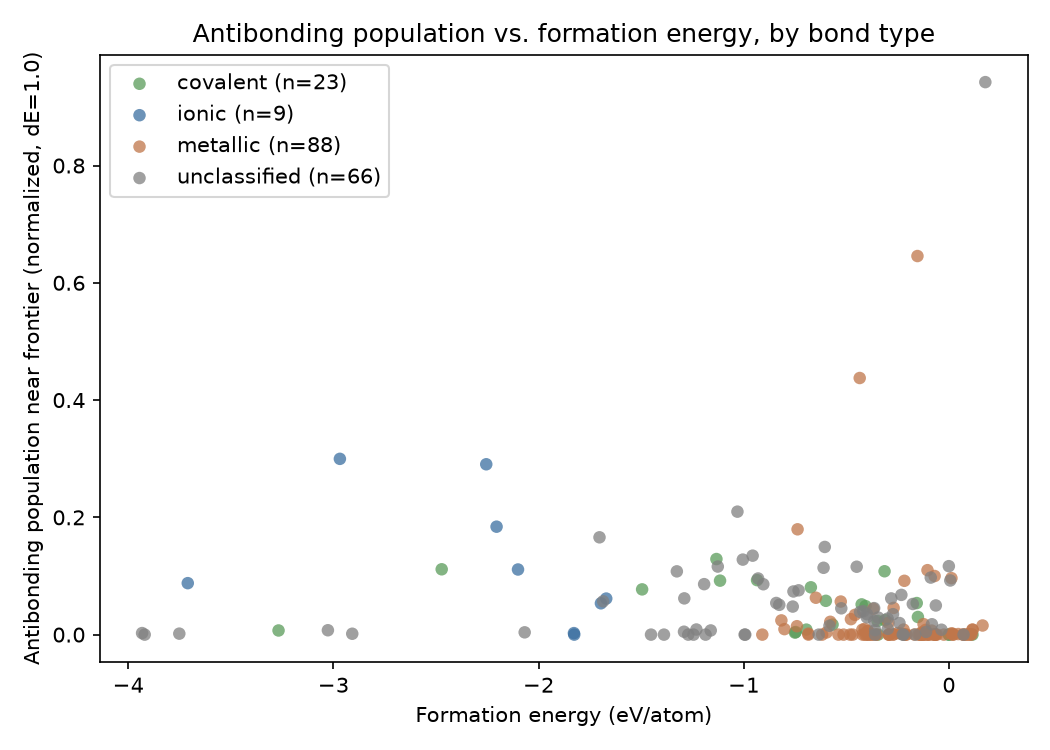
\includegraphics[width=0.75\textwidth]{antibonding_vs_formation_energy_by_bondtype.png}
\end{center}

\textbf{Mission \#5 (reaction ICOHP)}: $\rho=0.502$, $p=6.3\times10^{-19}$
($n=275$) --- up from $\rho=0.370$, and now the clear strongest
correlation in the project by a wider margin than before.
\texttt{bond\_type} stratification still fully explains that layer of the
pooled signal (Kruskal--Wallis $p=1.1\times10^{-15}$, no stratum
survives) --- \textbf{but \texttt{is\_metal} stratification now survives
on both sides} (\texttt{is\_metal=False}: $\rho=0.319$, $p=0.0001$;
\texttt{is\_metal=True}: $\rho=0.256$, $p=0.0025$), where at $n=186$
neither did. This revises the previous verdict that "the between-group
confound explains the entirety of the observable signal" --- it explains
the \texttt{bond\_type}-level pooling completely, but not a real,
newly-detectable within-\texttt{is\_metal}-group relationship. Case 2
(polymorph comparison), extended from 8 to \textbf{49 groups} specifically
because \texttt{extension4} was designed to fix that sampling gap:
53.1\% agreement between most-bonding and most-stable member, an exact
Poisson-binomial test against the 45.9\% chance baseline gives $P=0.19$
--- still no signal, but now a real test instead of an 8-point
exploratory pass.

\begin{center}

\includegraphics[width=0.75\textwidth]{reaction_icohp_vs_formation_energy_per_atom_by_bondtype.png}
\end{center}

\textbf{Still no SISSO.} Reaction ICOHP is now the strongest raw
correlate of \texttt{formation\_energy\_per\_atom} in the project, and
the first descriptor whose signal is not fully explained away by
between-group clustering at every level tested --- the strongest
argument yet for a stratified (\texttt{is\_metal}-conditional) feature
search over a pooled one, still not attempted.

\noindent\textit{Detailed reports:}
\texttt{analysis/REPORT\_antibonding.md}, \texttt{analysis/REPORT\_reaction\_icohp.md}.
The diagnosis of mission \#3's (min-cut) collapse is in
Appendix~\ref{sec:appendix-percolation}
(\texttt{analysis/REPORT\_dimensionality\_mincut.md}).

\section{Project Reframing (August 16): the Central Question is $\Delta$(ICOHP)-Based Viability}
\label{sec:reframing}

\textbf{The project's central research question is restated as of this
update: does $\Delta$(ICOHP) --- the reaction-ICOHP descriptor for a
compound's decomposition into elements, and specifically the sign-based
endobondic/exobondic classification it supports --- distinguish
thermodynamically stable, metastable, and unstable compounds?} This
supersedes the percolation-weight-centric framing that organized the
original campaign 2 (Appendix~\ref{sec:appendix-percolation}) ---
percolation weight (mission \#1) and network dimensionality/periodic
min-cut (mission \#3) remain valuable as the historical foundation
(periodic graph construction, the statistical conventions every later
mission still reuses) but are no longer this project's organizing
question, consistent with min-cut's own headline correlation not
surviving the dataset's growth to 349 compounds (\S\ref{sec:followups2},
Appendix~\ref{sec:appendix-percolation}). Full detail:
\texttt{analysis/REPORT\_delta\_icohp\_viability.md},
\texttt{analysis/test\_delta\_icohp\_viability.py}.

\subsection{Reference concordance, formalized}

\S\ref{sec:followups2} already showed all 7 reference reactions
reproducing to within a few kJ/mol. Correlation alone (Pearson/Spearman)
is not the right test for "do our numbers match the reference values" ---
it is satisfied by any monotonic relationship, even one with a large
systematic offset or scale factor. \textbf{Lin's Concordance Correlation
Coefficient} (CCC) specifically tests agreement with the identity line
(computed = reference), the actual claim being tested:

\begin{center}
\begin{tabular}{@{}lr@{}}
\toprule
Statistic & Value \\
\midrule
$n$ & 7 \\
Lin's CCC & \textbf{0.999998} \\
Pearson $r$ & 0.999999 ($p=3.5\times10^{-15}$) \\
Sign agreement & 7/7 \\
Mean $|$residual$|$ & 0.76 kJ/mol \\
Max $|$residual$|$ & 1.70 kJ/mol \\
RMSE & 0.98 kJ/mol \\
\bottomrule
\end{tabular}
\end{center}

A CCC this close to 1 means the two methods agree essentially within the
reference values' own reporting precision (rounded to 2--3 decimals),
not merely that they move together --- the implementation is validated
by it, not just individually spot-checked.

\subsection{Extended to every compound computed to date, pooled without regard to campaign}

\textbf{Deliberately not organized by which historical campaign or
extension batch a compound came from} --- those boundaries reflect
submission order across sessions, not chemistry, and grouping by them
would itself be exactly the kind of between-group confound this
project's methodology exists to catch (the same lesson
Appendix~\ref{sec:appendix-percolation}'s min-cut diagnosis already
demonstrated). \textbf{281 case-1 reactions}, every element and compound
with a computed decomposition-into-elements reaction across the whole
project, pooled into one population.

\textbf{Continuous stability targets:}

\begin{center}
\begin{tabular}{@{}lrrr@{}}
\toprule
Target & $n$ & $\rho$ & $p$ \\
\midrule
\texttt{formation\_energy\_per\_atom} & 275 & $-0.5016$ & $6.3\times10^{-19}$ \\
\texttt{energy\_above\_hull\_eV\_per\_atom} & 279 & $-0.1096$ & $0.068$ \\
\bottomrule
\end{tabular}
\end{center}

(Sign: \texttt{reaction\_analysis}'s products$-$reactants convention,
opposite \texttt{reaction\_icohp.py}'s own column reported elsewhere in
this report --- same magnitude, flipped sign.) The formation-energy
result is the same relationship as \S\ref{sec:followups2}'s mission-\#5
headline, confirmed here on the pooled, campaign-agnostic population.

\textbf{Sign-based (endobondic/exobondic) discrimination.} Experimental-
viability proxy (a compound's \texttt{theoretical} flag: \texttt{False}
means it has been experimentally realized):

\begin{center}
\begin{tabular}{@{}lrr@{}}
\toprule
 & endobondic & exobondic \\
\midrule
experimental ($n=177$) & 47 & 130 \\
theoretical-only ($n=98$) & 17 & 81 \\
\bottomrule
\end{tabular}
\end{center}

Fisher's exact test: $p=0.10$, odds ratio $=1.72$ (endobondic is $\sim
1.7\times$ more common among experimentally-realized compounds --- the
expected direction, since endobondic is meant as a kinetic-barrier
signature --- but not significant at this sample size).

\textbf{Finer-grained (family, three-way, $n=175$):}

\begin{center}
\begin{tabular}{@{}lrrr@{}}
\toprule
family & $n$ & median $\Delta$ICOHP/atom (eV) & \% endobondic \\
\midrule
exp\_metastable & 59 & $-1.077$ & \textbf{27.1\%} \\
exp\_stable & 59 & $-1.589$ & 20.3\% \\
theo\_metastable & 59 & $-1.659$ & \textbf{11.9\%} \\
\bottomrule
\end{tabular}
\end{center}

Kruskal--Wallis across the three groups: $H=2.81$, $p=0.245$ ---
\textbf{not significant}, but the ordering is exactly the physically-
motivated one: \texttt{exp\_metastable} compounds (known to exist
despite sitting off the convex hull --- the category the
endobondic/exobondic framework is specifically about) have the highest
endobondic fraction; \texttt{theo\_metastable} compounds (never
synthesized) have the lowest.

\subsection{Reading}

The 7 reference reactions reproduce essentially exactly --- the
implementation is correct. Extending the same sign-based logic to a
much larger, more heterogeneous, and generally much more comfortably
stable population does not yet produce a statistically significant
stable/metastable/unstable discriminator, though every trend points the
right way. This is not a contradiction: the 7 reference cases were
chosen specifically as borderline-stability edge cases (Pb(N$_3$)$_2$,
S$_4$N$_2$/S$_4$N$_4$, ZnSn, Mn$_2$O$_7$) where a kinetic-barrier
explanation is specifically needed; most of this project's 281 compounds
are not that --- they are comfortably stable or comfortably not, where
the thermodynamic driving force (the formation-energy correlation above)
may simply dominate over the sign-based kinetic signal. \textbf{The
concrete next step}: extend deliberately to more borderline-stability
compounds, not just whatever the next unrelated mission happens to add
to the dataset. \texttt{classify.py}'s full \texttt{ViabilityLabel}
machinery (beyond the sign-only \texttt{BondingLabel} used here) needs
exactly such a population --- for the current dataset, decomposition
into elements is strongly exothermic for nearly every compound (normal
for stable inorganic chemistry), which would trivially classify almost
everything \texttt{STABLE\_ON\_HULL} and add no information beyond what
\texttt{energy\_above\_hull} already says directly.

\appendix

\section{Appendix: Percolation\_viability}
\label{sec:appendix-percolation}

This appendix collects everything related to the percolation weight and
its direct descendants (network dimensionality, periodic min-cut ---
missions \#1 and \#3): this was the central subject of the original
campaign 2, unmodified below from its first drafting, but it is no
longer this project's organizing question (\S\ref{sec:reframing}). The
corresponding source code has been moved to the repository's
\texttt{Percolation\_viability/} directory
(\texttt{percolation\_path.py}, \texttt{network\_dimensionality.py},
\texttt{periodic\_mincut.py}, and their tests
\texttt{tests/test\_percolation\_path.py},
\texttt{tests/test\_network\_dimensionality.py},
\texttt{tests/test\_periodic\_mincut.py}).

\subsection{Original objective (mission \#1)}

The very first report (6 toy compounds) established that the
percolation descriptor computed by \texttt{percolation\_path.py}
diverges sharply from classic ICOHP aggregates (sum, mean, min, max),
but without a sample large enough to statistically test whether that
difference is \emph{useful}: does the percolation descriptor carry
predictive information about thermodynamic stability
(\texttt{energy\_above\_hull}) that the classic aggregates don't already
carry? Campaign 2 built a 186-compound dataset (180 new + the 6 pilot
compounds) split into three families (\texttt{exp\_stable},
\texttt{exp\_metastable}, \texttt{theo\_metastable}, \S\ref{sec:dataset})
to settle that question.

\subsection{Original workflow diagram}

\begin{center}
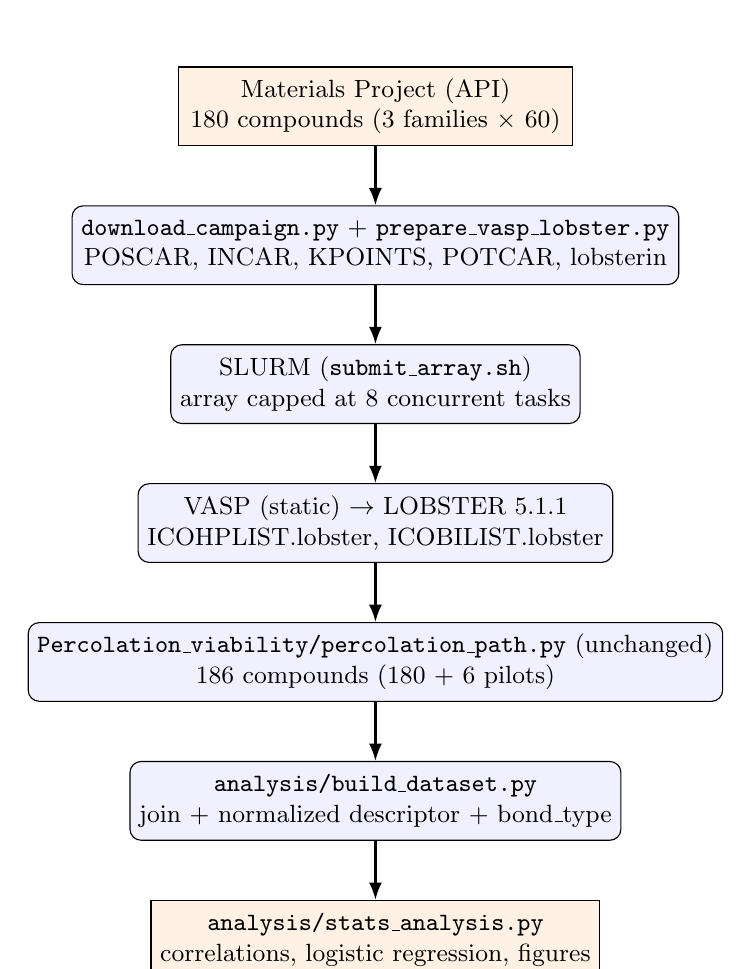
\begin{tikzpicture}[
  node distance=0.75cm and 1.6cm,
  box/.style={draw, rounded corners, minimum width=5.0cm, minimum height=1.0cm,
              align=center, fill=blue!6, font=\small},
  io/.style={draw, minimum width=5.0cm, minimum height=1.0cm, align=center,
             fill=orange!10, font=\small},
  arr/.style={-{Latex[length=2.2mm]}, thick}
]
\node[io]  (mp)     {Materials Project (API) \\ 180 compounds (3 families $\times$ 60)};
\node[box, below=of mp] (prep)   {\texttt{download\_campaign.py} + \texttt{prepare\_vasp\_lobster.py} \\ POSCAR, INCAR, KPOINTS, POTCAR, lobsterin};
\node[box, below=of prep] (slurm)  {SLURM (\texttt{submit\_array.sh}) \\ array capped at 8 concurrent tasks};
\node[box, below=of slurm] (vasplob) {VASP (static) $\rightarrow$ LOBSTER 5.1.1 \\ ICOHPLIST.lobster, ICOBILIST.lobster};
\node[box, below=of vasplob] (perc)   {\texttt{Percolation\_viability/percolation\_path.py} (unchanged) \\ 186 compounds (180 + 6 pilots)};
\node[box, below=of perc] (join)   {\texttt{analysis/build\_dataset.py} \\ join + normalized descriptor + bond\_type};
\node[io, below=of join] (stats)  {\texttt{analysis/stats\_analysis.py} \\ correlations, logistic regression, figures};

\draw[arr] (mp) -- (prep);
\draw[arr] (prep) -- (slurm);
\draw[arr] (slurm) -- (vasplob);
\draw[arr] (vasplob) -- (perc);
\draw[arr] (perc) -- (join);
\draw[arr] (join) -- (stats);
\end{tikzpicture}
\end{center}

\subsection{Campaign 2 dataset (186 compounds)}

\begin{center}
\begin{tabular}{@{}lrl@{}}
\toprule
Family & $n$ & $E_\text{hull}$ range (eV/atom) \\
\midrule
exp\_stable      & 63 & 0.0000 (by construction) \\
exp\_metastable  & 63 & 0.0005 -- 0.0907 \\
theo\_metastable & 60 & 0.0013 -- 0.1991 \\
\bottomrule
\end{tabular}

\vspace{0.3cm}

\begin{tabular}{@{}lr@{}}
\toprule
Bond type (\texttt{classify()}) & $n$ \\
\midrule
metallic       & 88 \\
covalent       & 23 \\
ionic          & 9 \\
unclassified   & 66 \\
\bottomrule
\end{tabular}
\end{center}

35\% of compounds (66/186) fall outside \texttt{classify()}'s three
categories --- mostly transition-metal pnictides/chalcogenides and
hydrogen-containing compounds. (Historical snapshot of campaign 2 alone;
the up-to-date table across the current 349 structures is in
\S\ref{sec:dataset}.)

\subsection{Results (with the percolation weight)}

\begin{center}
\small
\begin{tabular}{@{}llrrr@{}}
\toprule
Group & Metric & $n$ & $\rho$ & $p$ \\
\midrule
all & percolation weight (raw)        & 186 & 0.064 & 0.383 \\
all & percolation weight (normalized) & 186 & 0.071 & 0.339 \\
metallic & percolation weight (raw)        & 88 & 0.191 & 0.075 \\
metallic & percolation weight (normalized) & 88 & \textbf{0.222} & \textbf{0.038} \\
ionic$^*$ & percolation weight (raw)       & 9  & $-$0.402 & 0.284 \\
covalent & percolation weight (raw)        & 23 & 0.165 & 0.453 \\
\midrule
all & ICOHP sum    & 186 & 0.032 & 0.670 \\
all & ICOHP min    & 186 & 0.093 & 0.209 \\
metallic & ICOHP sum  & 88 & 0.223 & 0.037 \\
metallic & ICOHP min  & 88 & 0.198 & 0.065 \\
\bottomrule
\end{tabular}

\footnotesize $^*$ $n<15$: do not over-interpret.
\end{center}

In the one subgroup where any result reaches nominal significance
(metallic, $n=88$), the normalized percolation weight ($\rho=0.222$,
$p=0.038$) and the ICOHP sum ($\rho=0.223$, $p=0.037$) are statistically
indistinguishable in strength. \textbf{The percolation descriptor does
not demonstrate additional predictive power over the classic aggregates
on this dataset}.

\textbf{Reference logistic regression.} Stable (on-hull) vs. metastable,
features: normalized percolation weight, mean ICOHP, bond-type dummies
($n=120$ after dropping unclassified compounds).

\begin{center}
\begin{tabular}{@{}lr@{}}
\toprule
AUC (5-fold cross-validation) & $0.496 \pm 0.141$ \\
per-fold AUC & 0.556, 0.430, 0.252, 0.637, 0.607 \\
\bottomrule
\end{tabular}
\end{center}

AUC $\approx 0.5$: chance level. The wide spread across folds
(0.25--0.64) is itself informative: it indicates the absence of a stable,
learnable signal at this sample size, not merely a "weak but real" one.

\begin{center}
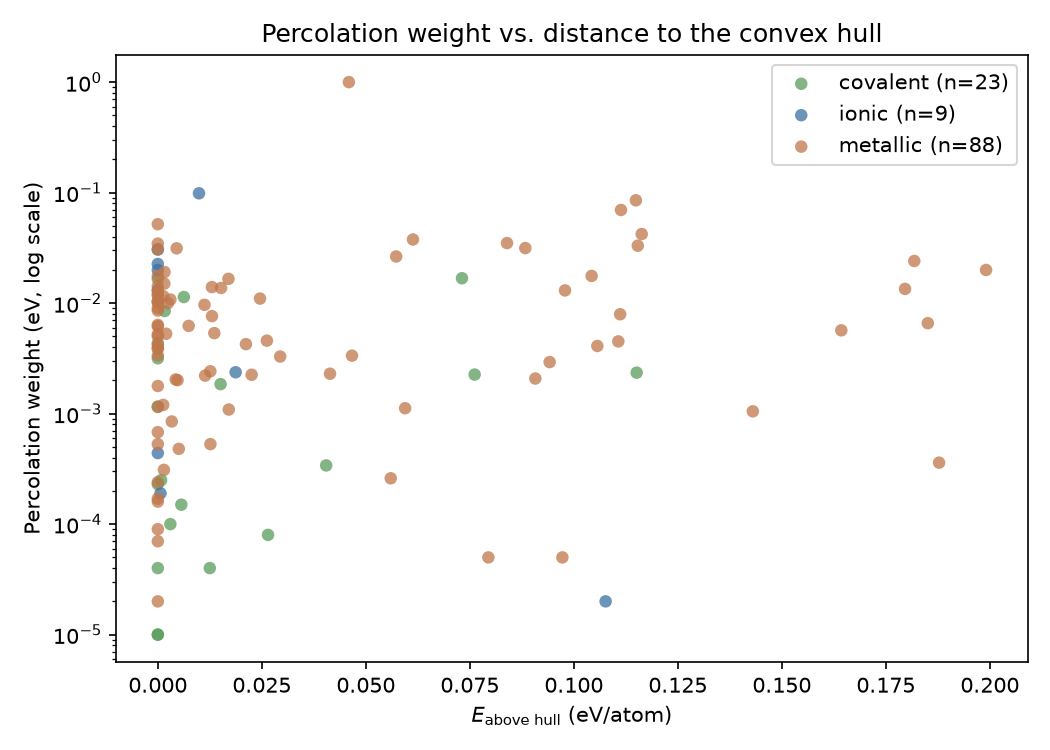
\includegraphics[width=0.85\textwidth]{percolation_vs_ehull.png}
\end{center}

\begin{center}

\includegraphics[width=0.55\textwidth]{roc_stable_vs_metastable.png}
\end{center}

\subsection{Mission \#3: network dimensionality and periodic min-cut}

Two new descriptors, \texttt{percolation\_path.py} left unchanged:
\texttt{network\_dimensionality.py} (0D--3D classification via a relative
bond-strength threshold + breadth-first search) and
\texttt{periodic\_mincut.py} (minimum cut via \texttt{networkx} max-flow,
separability rather than traversability). Headline: the normalized min-cut
is the \textbf{first descriptor in the project to reach a significant
global correlation} ($\rho=0.285$, $p=1.0\times10^{-4}$, $n=186$), likely
driven in part by between-bond-type clustering; dimensionality alone does
not separate \texttt{formation\_energy\_per\_atom}
(Kruskal--Wallis $p=0.19$).

\begin{center}
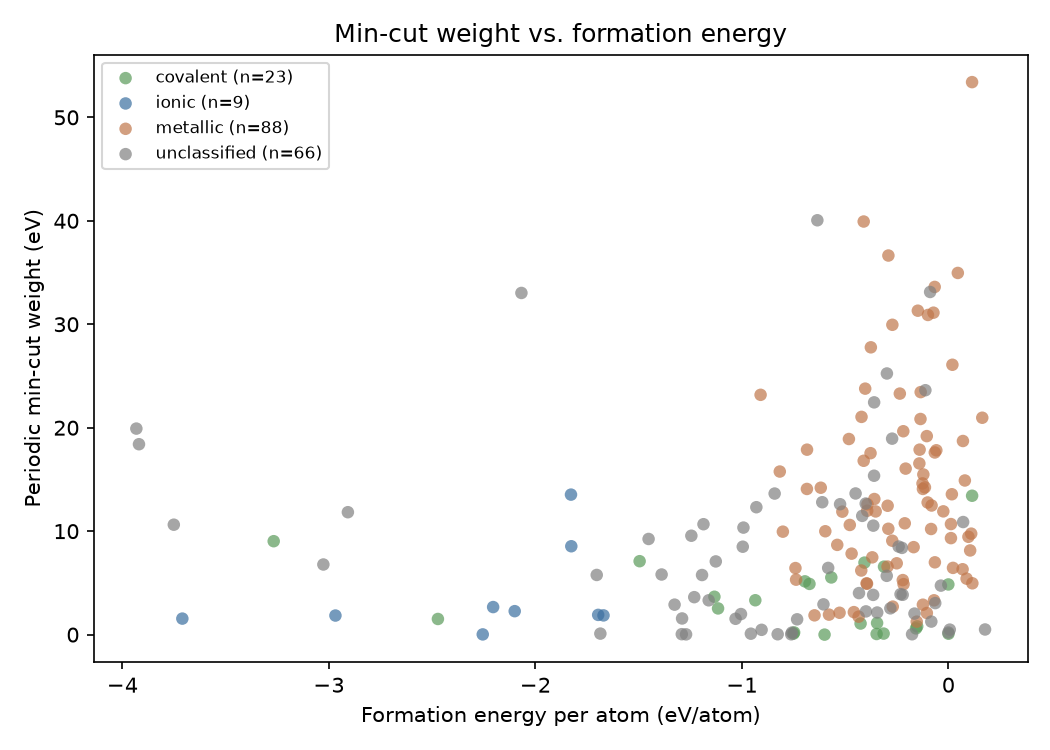
\includegraphics[width=0.75\textwidth]{mincut_vs_formation_energy.png}
\end{center}

\textbf{Why did the min-cut correlation collapse?} Mission \#3's
headline, $\rho=0.285$ at $n=186$, collapsed to $\rho=0.089$,
$p=0.098$ (not significant) at $n=349$. \textbf{This is not a refutation
of the original result} --- isolated, the original 186 compounds still
give $\rho=0.2845$, $p=8.3\times10^{-5}$, essentially identical to the
mission-\#3 number. The collapse is a dilution artifact from pooling
populations added for unrelated reasons:

\begin{itemize}
\item 65 of the 74 extension-batch-1--3 compounds are single-element
  reference structures (added for mission \#5's elemental references),
  sitting at \texttt{formation\_energy\_per\_atom}$\approx 0$ by
  construction with widely-scattered min-cut values --- mechanically
  dilutes a rank correlation regardless of any true relationship.
  Excluding them recovers $\rho=0.2157$ ($n=193$).
\item \texttt{extension4} is not one population but two, with
  \emph{opposite-sign} correlations: the experimental half is flat
  ($\rho=0.06$, not significant, $n=50$); the deliberately
  far-above-hull theoretical half shows a \emph{significant} correlation
  of the \emph{opposite} sign ($\rho=-0.40$, $p=0.011$, $n=39$) --- a
  higher min-cut there is associated with a \emph{more} negative
  (more stable) formation energy, the reverse of the original
  population's trend.
\end{itemize}

\begin{center}
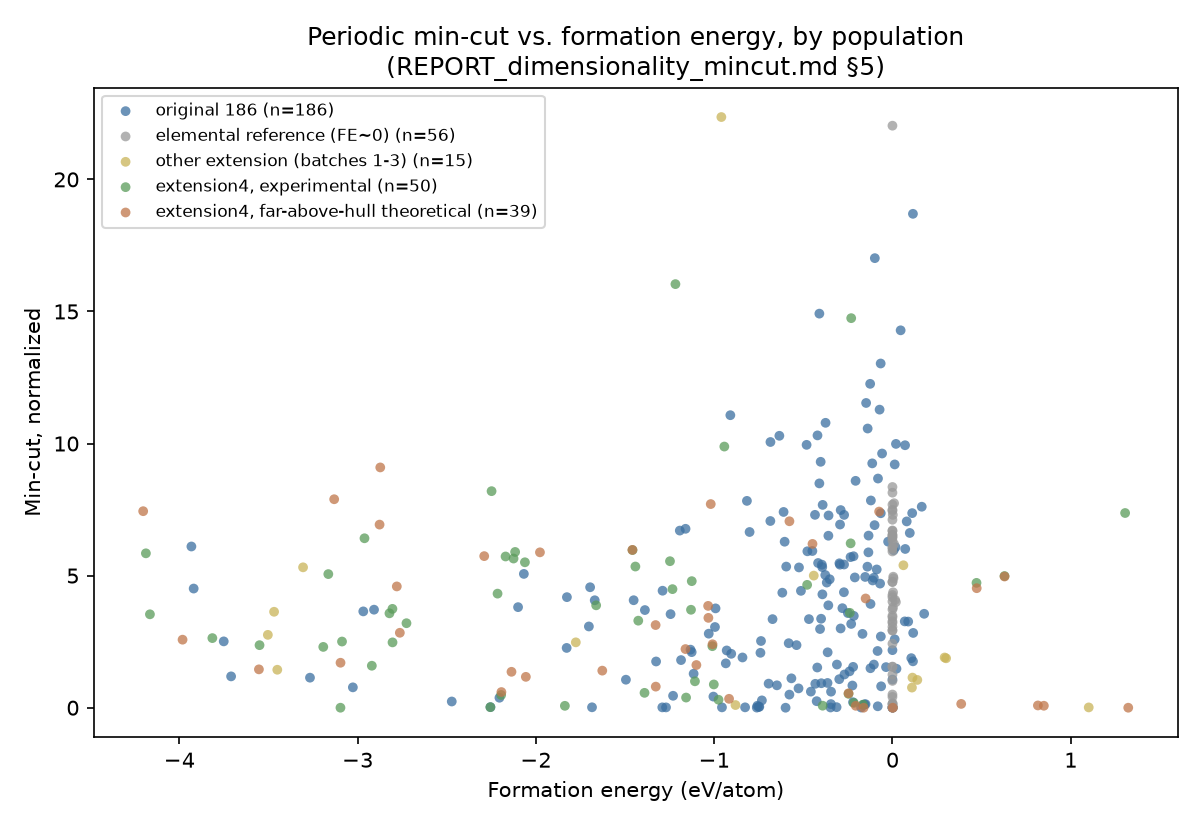
\includegraphics[width=0.85\textwidth]{mincut_vs_formation_energy_by_population.png}
\end{center}

\textbf{This opposite sign is itself resolved} (August-16 follow-up,
four independent checks on the 39 \texttt{theo\_far\_hull} compounds,
\texttt{analysis/investigate\_theo\_far\_hull\_signflip.py}): neither a
cell-size/symmetry selection artifact (survives controlling for
\texttt{n\_sites}+\texttt{sg\_number}, $\rho=-0.39$) nor a real physical
effect of far-from-hull structures, but a \textbf{between-anion-chemistry
confound} --- F-containing systems (high min-cut, strongly negative
formation energy) and azide N$_3$-containing systems (near-zero min-cut,
near-zero/positive formation energy) pull the pooled correlation in
opposite directions. Controlling for anion identity (dummy regression,
$n=39$) or comparing the experimental/theoretical pair within the exact
same chemical system ($n=37$ pairs) both independently collapse the
correlation to $\rho\approx-0.07$, not significant --- the same
between-group clustering failure mode this project has now hit three
times (min-cut/\texttt{bond\_type}, antibonding/\texttt{is\_metal}, and
now min-cut/anion).

\textbf{Recommendation}: any future min-cut-vs-formation-energy number
(or, by the same logic, any other descriptor's) should be conditioned on
\texttt{family}/selection-provenance, the same way this project already
conditions on \texttt{bond\_type}/\texttt{is\_metal}.

\subsection{Limits specific to the percolation weight}

\begin{itemize}
  \item \textbf{Primitive vs. conventional cell}: not reprocessed on the
    186-compound dataset. Most likely explanation for the weak observed
    correlations --- the strongest bond can sit entirely inside the
    primitive cell and contribute to no non-contractile cycle at all,
    biasing the measured "weakest link." Tested on the 6 pilot compounds
    (mission \#2): the choice changes the percolation weight
    substantially (3x-55x) but in the \emph{opposite} direction from the
    hypothesis (the weight gets \emph{smaller} with a larger cell); not
    extended to the full dataset based on this result.
  \item \textbf{Chance-level reference logistic regression}
    (AUC $\approx 0.5$) with percolation weight as a feature.
  \item \textbf{Why not SISSO}: a single candidate descriptor (the
    percolation weight, in two algebraically related variants), compared
    against aggregates that are themselves functions of the same
    underlying ICOHP values --- no meaningful combinatorial search space
    at this stage.
\end{itemize}

\subsection{Conclusion of the original campaign}

The 186-compound dataset was built, computed (VASP+LOBSTER), and
analyzed end to end. The headline result is a \emph{negative} but
quantified and honest one: at this sample size, the percolation
descriptor shows no significant correlation with thermodynamic
stability, and demonstrates no advantage over classic ICOHP aggregates.
This result, together with the min-cut result (mission \#3), motivated
the project's reframing around $\Delta$(ICOHP) documented in
\S\ref{sec:reframing}.

\subsection{Compound List (percolation weight)}

Campaign 2's 186 compounds, grouped by category (family), with their
Materials Project identifier, PBE thermodynamic hull distance
(\texttt{energy\_above\_hull}), and the minimum ICOHP percolation weight
(\texttt{icohp\_percolation\_weight\_min}). Auto-generated from
\texttt{analysis/percolation\_vs\_hull.csv} by
\texttt{report/gen\_appendix.py}.

{\small
\begin{longtable}{@{}l l l r r@{}}
\caption{Complete list of the 186 compounds, grouped by category, with their Materials Project identifier, PBE hull distance, and minimum ICOHP percolation weight.}\label{tab:appendix-compounds}\\
\toprule
Formula & mp-id & Bonding & $E_\text{hull}$ (eV/at) & Percolation weight (eV) \\
\midrule
\endfirsthead
\multicolumn{5}{@{}l}{\tablename\ \thetable\ (continued)}\\
\toprule
Formula & mp-id & Bonding & $E_\text{hull}$ (eV/at) & Percolation weight (eV) \\
\midrule
\endhead
\bottomrule
\endfoot
\multicolumn{5}{@{}l}{\textbf{Experimental, stable (hull)} ($n=63$)} \\
\midrule
As$_{2}$S$_{3}$ & mp-1189572 & covalent & 0.0000 & 1.00e-05 \\
AsF$_{3}$ & mp-28027 & covalent & 0.0000 & 0.00e+00 \\
BI$_{3}$ & mp-23189 & covalent & 0.0000 & 1.00e-05 \\
BW & mp-7832 & -- & 0.0000 & 1.90e-04 \\
BaAu$_{2}$ & mp-30363 & metallic & 0.0000 & 5.19e-02 \\
BaCl$_{2}$ & mp-568662 & ionic & 0.0000 & 1.31e-02 \\
BaH$_{2}$ & mp-23715 & -- & 0.0000 & 2.40e-04 \\
Be$_{2}$Cu & mp-2031 & metallic & 0.0000 & 1.15e-03 \\
Be$_{2}$Nb$_{3}$ & mp-11272 & metallic & 0.0000 & 6.36e-03 \\
Be$_{2}$V & mp-11281 & metallic & 0.0000 & 6.80e-04 \\
CaAl$_{4}$ & mp-1749 & metallic & 0.0000 & 1.03e-02 \\
CaSn & mp-2450 & metallic & 0.0000 & 5.23e-03 \\
CdPd & mp-1696 & metallic & 0.0000 & 9.00e-05 \\
CoB & mp-20857 & -- & 0.0000 & 6.00e-05 \\
Cs$_{2}$As$_{3}$ & mp-15557 & -- & 0.0000 & 2.02e-02 \\
FeS & mp-505531 & -- & 0.0000 & 3.05e-03 \\
Ge$_{2}$Os & mp-10032 & metallic & 0.0000 & 1.21e-02 \\
HfTc$_{2}$ & mp-1095669 & metallic & 0.0000 & 1.77e-02 \\
Hg$_{4}$Pt & mp-936 & metallic & 0.0000 & 3.36e-03 \\
HgF$_{2}$ & mp-8177 & -- & 0.0000 & 8.95e-03 \\
InBr & mp-22870 & covalent & 0.0000 & 1.02e-02 \\
KI & mp-22898 & ionic & 0.0000 & 2.26e-02 \\
KN$_{3}$ & mp-827 & -- & 0.0000 & 2.80e-04 \\
Li$_{2}$Se & mp-2286 & -- & 0.0000 & 1.16e-02 \\
LiB & mp-1001835 & -- & 0.0000 & 2.91e-03 \\
Mg$_{2}$Ni & mp-2137 & metallic & 0.0000 & 1.60e-04 \\
MgP$_{4}$ & mp-384 & -- & 0.0000 & 0.00e+00 \\
MnAl$_{12}$ & mp-1104165 & metallic & 0.0000 & 1.42e-02 \\
MoSe$_{2}$ & mp-1634 & covalent & 0.0000 & 1.16e-03 \\
NaS & mp-2400 & -- & 0.0000 & 0.00e+00 \\
Na & mp-10172 & -- & 0.0000 & 1.97e-03 \\
Nb$_{3}$Ir & mp-1458 & metallic & 0.0000 & 9.02e-03 \\
NbGa$_{3}$ & mp-1973 & metallic & 0.0000 & 8.58e-03 \\
PI$_{2}$ & mp-29443 & covalent & 0.0000 & 2.30e-04 \\
PbSe & mp-2201 & covalent & 0.0000 & 1.66e-02 \\
RbI & mp-22903 & ionic & 0.0000 & 2.00e-02 \\
Sc$_{5}$Ge$_{3}$ & mp-17190 & metallic & 0.0000 & 5.30e-04 \\
ScAg$_{2}$ & mp-1018128 & metallic & 0.0000 & 1.70e-04 \\
ScTe & mp-10026 & -- & 0.0000 & 7.12e-03 \\
SnPt & mp-19856 & metallic & 0.0000 & 1.29e-02 \\
SrO$_{2}$ & mp-2697 & ionic & 0.0000 & 4.40e-04 \\
SrSi & mp-2661 & metallic & 0.0000 & 7.00e-05 \\
Ta$_{5}$Ge$_{3}$ & mp-17593 & metallic & 0.0000 & 3.46e-02 \\
TaP & mp-1067587 & -- & 0.0000 & 3.14e-02 \\
TaSb$_{2}$ & mp-11697 & metallic & 0.0000 & 1.17e-02 \\
Te$_{2}$Pd & mp-782 & -- & 0.0000 & 1.44e-02 \\
Te$_{2}$Ru & mp-267 & covalent & 0.0000 & 4.34e-03 \\
TeO$_{2}$ & mp-8377 & covalent & 0.0000 & 4.00e-05 \\
Ti$_{3}$In & mp-866046 & metallic & 0.0000 & 5.01e-03 \\
Ti$_{3}$Pt & mp-2339 & metallic & 0.0000 & 1.78e-03 \\
TiBe$_{12}$ & mp-1104067 & metallic & 0.0000 & 2.40e-04 \\
TiNi & mp-1048 & metallic & 0.0000 & 3.91e-03 \\
TiO & mp-1071163 & -- & 0.0000 & 6.40e-04 \\
TiSi$_{2}$ & mp-1077503 & metallic & 0.0000 & 6.18e-03 \\
TlCl & mp-571079 & -- & 0.0000 & 7.17e-03 \\
VNi$_{2}$ & mp-11531 & metallic & 0.0000 & 3.88e-03 \\
WO$_{2}$ & mp-1524394 & -- & 0.0000 & 2.20e-04 \\
Zr$_{2}$Au & mp-2348 & metallic & 0.0000 & 3.06e-02 \\
Zr$_{5}$Pb$_{3}$ & mp-681992 & metallic & 0.0000 & 2.00e-05 \\
ZrMo$_{2}$ & mp-2049 & metallic & 0.0000 & 1.05e-02 \\
Si & mp-149 & covalent & 0.0000 & 3.17e-03 \\
NaCl & mp-22862 & ionic & 0.0000 & 3.07e-02 \\
AlNi & mp-1487 & metallic & 0.0000 & 4.19e-03 \\
\midrule
\multicolumn{5}{@{}l}{\textbf{Experimental, metastable} ($n=63$)} \\
\midrule
CdI$_{2}$ & mp-567259 & -- & 0.0005 & 2.38e-02 \\
MgCl$_{2}$ & mp-570259 & ionic & 0.0006 & 1.90e-04 \\
C & mp-169 & covalent & 0.0008 & 2.50e-04 \\
ZrBr & mp-1065846 & -- & 0.0008 & 7.88e-03 \\
Li$_{3}$Hg & mp-1646 & metallic & 0.0013 & 1.20e-03 \\
Ta$_{7}$Co$_{6}$ & mp-1104548 & metallic & 0.0015 & 3.10e-04 \\
CaGa$_{4}$ & mp-2461 & metallic & 0.0016 & 1.91e-02 \\
InCl & mp-571636 & covalent & 0.0016 & 8.50e-03 \\
NiB & mp-14019 & -- & 0.0018 & 4.10e-04 \\
MgH$_{2}$ & mp-23711 & -- & 0.0019 & 1.00e-05 \\
Sn$_{7}$Ir$_{5}$ & mp-20466 & metallic & 0.0024 & 1.00e-02 \\
NaN$_{3}$ & mp-1066400 & -- & 0.0029 & 7.00e-04 \\
ClF$_{3}$ & mp-556767 & -- & 0.0030 & 0.00e+00 \\
SiS$_{2}$ & mp-1095294 & covalent & 0.0030 & 1.00e-04 \\
Sr$_{5}$Sn$_{3}$ & mp-17720 & metallic & 0.0030 & 1.08e-02 \\
Te$_{2}$Ir & mp-1551 & -- & 0.0030 & 2.80e-03 \\
Li$_{13}$Sn$_{5}$ & mp-30769 & metallic & 0.0033 & 8.50e-04 \\
H$_{3}$N & mp-643432 & covalent & 0.0038 & 0.00e+00 \\
Cs$_{2}$Se & mp-1011696 & -- & 0.0042 & 2.62e-02 \\
In$_{3}$Ir & mp-630976 & metallic & 0.0043 & 2.04e-03 \\
HI & mp-697025 & -- & 0.0044 & 0.00e+00 \\
Rb$_{2}$Hg$_{7}$ & mp-31474 & metallic & 0.0045 & 3.14e-02 \\
PbAu$_{2}$ & mp-19871 & metallic & 0.0047 & 2.01e-03 \\
BeCu & mp-2323 & metallic & 0.0050 & 4.80e-04 \\
SiO$_{2}$ & mp-546794 & covalent & 0.0056 & 1.50e-04 \\
IF$_{7}$ & mp-27988 & -- & 0.0063 & 0.00e+00 \\
K & mp-10157 & -- & 0.0069 & 8.07e-02 \\
Al$_{3}$Os$_{2}$ & mp-16521 & metallic & 0.0074 & 6.23e-03 \\
Nb$_{2}$O$_{5}$ & mp-1595 & -- & 0.0075 & 1.00e-04 \\
LiBr & mp-23259 & ionic & 0.0099 & 9.88e-02 \\
ZnAg & mp-1912 & metallic & 0.0112 & 9.67e-03 \\
MgPd$_{3}$ & mp-7753 & metallic & 0.0114 & 2.21e-03 \\
AsPd$_{2}$ & mp-1080831 & -- & 0.0118 & 3.50e-04 \\
GeSe$_{2}$ & mp-10074 & covalent & 0.0125 & 4.00e-05 \\
Re$_{3}$Ge$_{7}$ & mp-29141 & metallic & 0.0126 & 2.42e-03 \\
Cu$_{3}$Ge & mp-19724 & metallic & 0.0126 & 5.30e-04 \\
Ti$_{3}$Ge & mp-1189044 & metallic & 0.0130 & 1.40e-02 \\
ZrGa$_{3}$ & mp-30685 & metallic & 0.0130 & 7.64e-03 \\
SrAl$_{2}$ & mp-1638 & metallic & 0.0136 & 5.36e-03 \\
NiS & mp-1547 & -- & 0.0142 & 3.00e-04 \\
Al$_{12}$W & mp-11227 & metallic & 0.0152 & 1.37e-02 \\
CsH & mp-632319 & -- & 0.0161 & 2.66e-02 \\
CaGa$_{2}$ & mp-992 & metallic & 0.0170 & 1.66e-02 \\
NiHg$_{4}$ & mp-570835 & metallic & 0.0171 & 1.09e-03 \\
SiRh & mp-2287 & metallic & 0.0246 & 1.10e-02 \\
BaSn$_{5}$ & mp-571353 & metallic & 0.0262 & 4.58e-03 \\
PS & mp-612 & covalent & 0.0265 & 8.00e-05 \\
AsRh & mp-22079 & -- & 0.0269 & 1.93e-03 \\
Te$_{2}$Au & mp-567525 & -- & 0.0274 & 1.62e-02 \\
Be$_{3}$N$_{2}$ & mp-6977 & -- & 0.0315 & 2.00e-05 \\
Y$_{2}$O$_{3}$ & mp-558573 & -- & 0.0342 & 5.00e-05 \\
AgO & mp-1079720 & -- & 0.0423 & 4.00e-05 \\
FeTe$_{2}$ & mp-1102002 & -- & 0.0449 & 5.20e-04 \\
H$_{2}$O & mp-2739191 & -- & 0.0494 & 0.00e+00 \\
CdO$_{2}$ & mp-2310 & -- & 0.0562 & 9.00e-05 \\
Mo$_{3}$Se$_{4}$ & mp-21021 & -- & 0.0609 & 1.84e-03 \\
PbSe & mp-22009 & covalent & 0.0731 & 1.68e-02 \\
Be$_{12}$Pd & mp-12666 & metallic & 0.0795 & 5.00e-05 \\
Sr$_{2}$As & mp-15697 & -- & 0.0800 & 2.06e-03 \\
AsRh$_{2}$ & mp-1102364 & -- & 0.0806 & 4.63e-03 \\
ZrRh & mp-2808 & metallic & 0.0839 & 3.50e-02 \\
K$_{2}$S & mp-559278 & -- & 0.0873 & 1.07e-02 \\
Ge$_{4}$Rh & mp-1104286 & metallic & 0.0907 & 2.08e-03 \\
\midrule
\multicolumn{5}{@{}l}{\textbf{Theoretical, metastable} ($n=60$)} \\
\midrule
Li$_{3}$Ag & mp-976408 & metallic & 0.0013 & 1.15e-02 \\
Y$_{3}$Co & mp-1189329 & metallic & 0.0016 & 1.50e-02 \\
TiNi & mp-1067248 & metallic & 0.0020 & 5.29e-03 \\
TaP & mp-1187244 & -- & 0.0033 & 3.59e-02 \\
Sr$_{3}$As$_{4}$ & mp-678007 & -- & 0.0062 & 4.47e-03 \\
Ga$_{2}$Se$_{3}$ & mp-1224809 & covalent & 0.0063 & 1.14e-02 \\
MnN & mp-1009130 & covalent & 0.0151 & 1.85e-03 \\
BeCl$_{2}$ & mp-1190080 & ionic & 0.0187 & 2.37e-03 \\
MgSn & mp-1094801 & metallic & 0.0212 & 4.26e-03 \\
TiW & mp-1216621 & metallic & 0.0225 & 2.25e-03 \\
SrTl$_{3}$ & mp-1206636 & metallic & 0.0294 & 3.29e-03 \\
IrCl$_{3}$ & mp-729507 & -- & 0.0301 & 2.72e-03 \\
Ta$_{4}$C$_{3}$ & mp-1218000 & -- & 0.0335 & 1.44e-03 \\
Sc$_{2}$O$_{3}$ & mp-755313 & -- & 0.0364 & 5.10e-04 \\
SnBr$_{2}$ & mp-978985 & covalent & 0.0405 & 3.40e-04 \\
Sn$_{7}$Pd$_{5}$ & mp-1219006 & metallic & 0.0414 & 2.30e-03 \\
Tl$_{4}$Sn & mp-1216560 & metallic & 0.0459 & 1.00e+00 \\
LiTl$_{3}$ & mp-1185253 & metallic & 0.0467 & 3.35e-03 \\
PtCl$_{2}$ & mp-1219748 & -- & 0.0490 & 5.04e-03 \\
HCl & mp-684609 & -- & 0.0536 & 2.50e-04 \\
MgSn & mp-1094669 & metallic & 0.0560 & 2.60e-04 \\
K$_{5}$As$_{4}$ & mp-684799 & -- & 0.0564 & 8.80e-03 \\
KSn$_{3}$ & mp-1185151 & metallic & 0.0573 & 2.65e-02 \\
NbS$_{2}$ & mp-774873 & -- & 0.0576 & 1.20e-04 \\
YAg$_{3}$ & mp-1187811 & metallic & 0.0594 & 1.12e-03 \\
B$_{3}$Ir$_{2}$ & mp-1228647 & -- & 0.0609 & 2.80e-04 \\
TiMo$_{2}$ & mp-1216675 & metallic & 0.0613 & 3.77e-02 \\
Cr$_{2}$C & mp-1226378 & -- & 0.0625 & 2.08e-03 \\
ZrO$_{2}$ & mp-775909 & -- & 0.0627 & 1.20e-04 \\
Zn & mp-2647117 & -- & 0.0717 & 1.04e-02 \\
IN$_{2}$ & mp-1097011 & -- & 0.0730 & 4.70e-04 \\
CoSe$_{2}$ & mp-1390196 & -- & 0.0734 & 8.40e-04 \\
GeS & mp-12910 & covalent & 0.0762 & 2.26e-03 \\
ZrTi & mp-1215236 & metallic & 0.0883 & 3.15e-02 \\
VCo$_{3}$ & mp-1095057 & metallic & 0.0942 & 2.93e-03 \\
Tl$_{3}$Ga & mp-1187539 & metallic & 0.0972 & 5.00e-05 \\
CaGe$_{2}$ & mp-643542 & metallic & 0.0979 & 1.30e-02 \\
NbRh$_{2}$ & mp-1220414 & metallic & 0.1043 & 1.76e-02 \\
TcW & mp-1217337 & metallic & 0.1056 & 4.10e-03 \\
MgF$_{2}$ & mp-560236 & ionic & 0.1076 & 2.00e-05 \\
VN & mp-1017532 & -- & 0.1080 & 4.00e-05 \\
Na$_{2}$Cl & mp-990084 & -- & 0.1105 & 3.76e-02 \\
ZnPb$_{3}$ & mp-1187949 & metallic & 0.1107 & 4.51e-03 \\
Sr$_{3}$Sn & mp-1187136 & metallic & 0.1111 & 7.94e-03 \\
TaRe & mp-1217894 & metallic & 0.1113 & 6.98e-02 \\
Al$_{4}$Si & mp-1228120 & metallic & 0.1149 & 8.54e-02 \\
B$_{6}$Pb & mp-1096825 & covalent & 0.1151 & 2.35e-03 \\
ScTc$_{3}$ & mp-867262 & metallic & 0.1154 & 3.31e-02 \\
CrMo & mp-1226200 & metallic & 0.1163 & 4.23e-02 \\
BPd$_{5}$ & mp-1228665 & -- & 0.1325 & 2.42e-02 \\
Zr$_{3}$Be & mp-1188016 & metallic & 0.1430 & 1.05e-03 \\
Na$_{3}$Cl & mp-1064484 & -- & 0.1456 & 2.55e-03 \\
SiAu$_{3}$ & mp-1186998 & metallic & 0.1643 & 5.68e-03 \\
InSe$_{2}$ & mp-1232036 & -- & 0.1733 & 1.64e-03 \\
TiSi$_{2}$ & mp-570991 & metallic & 0.1796 & 1.35e-02 \\
BeAu$_{3}$ & mp-983539 & metallic & 0.1818 & 2.41e-02 \\
Zr$_{3}$Ge & mp-1188039 & metallic & 0.1851 & 6.59e-03 \\
AlSb & mp-1023918 & metallic & 0.1878 & 3.60e-04 \\
Mg$_{15}$B & mp-1023515 & -- & 0.1943 & 2.80e-04 \\
HfMo & mp-1224314 & metallic & 0.1991 & 2.00e-02 \\
\midrule
\end{longtable}
}

\section{VASP Calculation Parameters}
\label{sec:appendix-incar}

Fixed INCAR parameters, identical across campaign 2's 186 compounds
(static, LOBSTER-compatible run) --- only \texttt{NBANDS}
(appendix~\ref{sec:appendix-kpoints}) and the k-point grid vary by
compound. Same settings applied to the four \texttt{extension} batches
(\S\ref{sec:followups2}).

\begin{center}
\input{appendix_dft_common_en.tex}
\end{center}

\section{PAW-PBE Potentials}

One PAW-PBE potential per element present in the dataset (pymatgen's
\texttt{MPRelaxSet} library --- the same one Materials Project used to
relax the input structures), with one documented exception for tungsten
(\S8): the recommended \texttt{W\_pv} variant is absent from the local
mirror, and \texttt{W\_sv} turned out to be corrupted (missing
\texttt{LEXCH} field) --- plain \texttt{W} is used instead, verified
valid.

{\small
\begin{longtable}{@{}l l@{}}
\caption{PAW-PBE potentials used, one per element present in the dataset (pymatgen's MPRelaxSet library, with one documented exception: W substituted for W\_pv/W\_sv, see \S7).}\\
\toprule
Element & PAW-PBE potential \\
\midrule
\endfirsthead
\toprule
Element & PAW-PBE potential \\
\midrule
\endhead
\bottomrule
\endfoot
Ag & \texttt{Ag (02Apr2005)} \\
Al & \texttt{Al (04Jan2001)} \\
As & \texttt{As (22Sep2009)} \\
Au & \texttt{Au (04Oct2007)} \\
B & \texttt{B (06Sep2000)} \\
Ba & \texttt{Ba\_sv (06Sep2000)} \\
Be & \texttt{Be\_sv (06Sep2000)} \\
Bi & \texttt{Bi (08Apr2002)} \\
Br & \texttt{Br (06Sep2000)} \\
C & \texttt{C (08Apr2002)} \\
Ca & \texttt{Ca\_sv (06Sep2000)} \\
Cd & \texttt{Cd (06Sep2000)} \\
Cl & \texttt{Cl (06Sep2000)} \\
Co & \texttt{Co (02Aug2007)} \\
Cr & \texttt{Cr\_pv (02Aug2007)} \\
Cs & \texttt{Cs\_sv (25Jan2019)} \\
Cu & \texttt{Cu\_pv (06Sep2000)} \\
F & \texttt{F (08Apr2002)} \\
Fe & \texttt{Fe\_pv (02Aug2007)} \\
Ga & \texttt{Ga\_d (06Jul2010)} \\
Ge & \texttt{Ge\_d (03Jul2007)} \\
H & \texttt{H (15Jun2001)} \\
Hf & \texttt{Hf\_pv (06Sep2000)} \\
Hg & \texttt{Hg (06Sep2000)} \\
I & \texttt{I (08Apr2002)} \\
In & \texttt{In\_d (06Sep2000)} \\
Ir & \texttt{Ir (06Sep2000)} \\
K & \texttt{K\_sv (06Sep2000)} \\
Li & \texttt{Li\_sv (10Sep2004)} \\
Mg & \texttt{Mg\_pv (13Apr2007)} \\
Mn & \texttt{Mn\_pv (02Aug2007)} \\
Mo & \texttt{Mo\_pv (04Feb2005)} \\
N & \texttt{N (08Apr2002)} \\
Na & \texttt{Na\_pv (19Sep2006)} \\
Nb & \texttt{Nb\_pv (08Apr2002)} \\
Ni & \texttt{Ni\_pv (06Sep2000)} \\
O & \texttt{O (08Apr2002)} \\
Os & \texttt{Os\_pv (20Jan2003)} \\
P & \texttt{P (06Sep2000)} \\
Pb & \texttt{Pb\_d (06Sep2000)} \\
Pd & \texttt{Pd (04Jan2005)} \\
Pt & \texttt{Pt (04Feb2005)} \\
Rb & \texttt{Rb\_sv (06Sep2000)} \\
Re & \texttt{Re\_pv (06Sep2000)} \\
Rh & \texttt{Rh\_pv (25Jan2005)} \\
Ru & \texttt{Ru\_pv (28Jan2005)} \\
S & \texttt{S (06Sep2000)} \\
Sb & \texttt{Sb (06Sep2000)} \\
Sc & \texttt{Sc\_sv (07Sep2000)} \\
Se & \texttt{Se (06Sep2000)} \\
Si & \texttt{Si (05Jan2001)} \\
Sn & \texttt{Sn\_d (06Sep2000)} \\
Sr & \texttt{Sr\_sv (07Sep2000)} \\
Ta & \texttt{Ta\_pv (07Sep2000)} \\
Tc & \texttt{Tc\_pv (04Feb2005)} \\
Te & \texttt{Te (08Apr2002)} \\
Ti & \texttt{Ti\_pv (07Sep2000)} \\
Tl & \texttt{Tl\_d (06Sep2000)} \\
V & \texttt{V\_pv (07Sep2000)} \\
W & \texttt{W (08Apr2002)} \\
Y & \texttt{Y\_sv (25May2007)} \\
Zn & \texttt{Zn (06Sep2000)} \\
Zr & \texttt{Zr\_sv (04Jan2005)} \\
\end{longtable}
}

\section{k-point Grid and NBANDS per Compound}
\label{sec:appendix-kpoints}

k-point grid auto-generated by
\texttt{pymatgen.io.vasp.Kpoints.automatic\_density\_by\_vol} (density
\texttt{kppvol=100}, $\Gamma$-centered or Monkhorst--Pack mesh depending
on cell symmetry) and \texttt{NBANDS}, derived per compound from the
number of local orbitals in the LOBSTER basis
(\texttt{Lobsterin.write\_INCAR}) --- a strictly sufficient value for the
local-basis projection, not a fixed guess.

{\small
\begin{longtable}{@{}l l l r@{}}
\caption{k-point grid (\texttt{pymatgen} automatic density, \texttt{kppvol=100}) and number of bands (derived from the LOBSTER basis) per compound.}\\
\toprule
Formula & mp-id & k-point grid & NBANDS \\
\midrule
\endfirsthead
\multicolumn{4}{@{}l}{\tablename\ \thetable\ (continued)}\\
\toprule
Formula & mp-id & k-point grid & NBANDS \\
\midrule
\endhead
\bottomrule
\endfoot
\multicolumn{4}{@{}l}{\textbf{Experimental, stable (hull)} ($n=63$)} \\
\midrule
As2S3 & mp-1189572 & 5 3 2 (G) & 80 \\
AsF3 & mp-28027 & 5 4 4 (G) & 64 \\
BI3 & mp-23189 & 4 4 4 (G) & 32 \\
BW & mp-7832 & 9 9 3 (G) & 52 \\
BaAu2 & mp-30363 & 6 6 7 (G) & 23 \\
BaCl2 & mp-568662 & 6 6 6 (G) & 13 \\
BaH2 & mp-23715 & 6 4 3 (G) & 28 \\
Be2Cu & mp-2031 & 7 7 7 (G) & 38 \\
Be2Nb3 & mp-11272 & 8 4 4 (M) & 74 \\
Be2V & mp-11281 & 7 7 4 (G) & 76 \\
CaAl4 & mp-1749 & 7 7 4 (G) & 21 \\
CaSn & mp-2450 & 6 6 4 (M) & 28 \\
CdPd & mp-1696 & 7 6 6 (G) & 36 \\
CoB & mp-20857 & 9 7 5 (G) & 52 \\
Cs2As3 & mp-15557 & 4 4 3 (G) & 44 \\
FeS & mp-505531 & 8 8 5 (G) & 26 \\
Ge2Os & mp-10032 & 9 6 4 (G) & 54 \\
HfTc2 & mp-1095669 & 5 5 3 (G) & 108 \\
Hg4Pt & mp-936 & 5 5 5 (G) & 45 \\
HgF2 & mp-8177 & 8 8 8 (G) & 17 \\
InBr & mp-22870 & 6 6 4 (M) & 26 \\
KI & mp-22898 & 6 6 6 (G) & 9 \\
KN3 & mp-827 & 5 5 5 (G) & 34 \\
Li2Se & mp-2286 & 7 7 7 (G) & 14 \\
LiB & mp-1001835 & 7 7 9 (G) & 18 \\
Mg2Ni & mp-2137 & 5 5 2 (G) & 102 \\
MgP4 & mp-384 & 5 5 3 (G) & 40 \\
MnAl12 & mp-1104165 & 4 4 4 (M) & 57 \\
MoSe2 & mp-1634 & 9 9 2 (G) & 34 \\
NaS & mp-2400 & 6 6 3 (G) & 32 \\
Na & mp-10172 & 8 8 4 (G) & 8 \\
Nb3Ir & mp-1458 & 5 5 5 (G) & 72 \\
NbGa3 & mp-1973 & 8 8 6 (M) & 36 \\
PI2 & mp-29443 & 6 4 3 (G) & 24 \\
PbSe & mp-2201 & 7 7 7 (G) & 13 \\
RbI & mp-22903 & 6 6 6 (G) & 9 \\
Sc5Ge3 & mp-17190 & 3 3 5 (G) & 154 \\
ScAg2 & mp-1018128 & 8 8 5 (G) & 28 \\
ScTe & mp-10026 & 7 7 4 (G) & 28 \\
SnPt & mp-19856 & 7 7 5 (G) & 36 \\
SrO2 & mp-2697 & 8 8 7 (G) & 13 \\
SrSi & mp-2661 & 7 6 4 (G) & 18 \\
Ta5Ge3 & mp-17593 & 4 4 4 (M) & 144 \\
TaP & mp-1067587 & 9 9 4 (G) & 26 \\
TaSb2 & mp-11697 & 8 5 4 (G) & 34 \\
Te2Pd & mp-782 & 7 7 5 (G) & 17 \\
Te2Ru & mp-267 & 7 5 4 (G) & 34 \\
TeO2 & mp-8377 & 6 5 3 (G) & 48 \\
Ti3In & mp-866046 & 5 5 6 (G) & 72 \\
Ti3Pt & mp-2339 & 5 5 5 (G) & 72 \\
TiBe12 & mp-1104067 & 7 5 5 (G) & 69 \\
TiNi & mp-1048 & 10 7 6 (G) & 36 \\
TiO & mp-1071163 & 10 6 6 (G) & 39 \\
TiSi2 & mp-1077503 & 8 8 4 (M) & 34 \\
TlCl & mp-571079 & 6 6 4 (M) & 26 \\
VNi2 & mp-11531 & 12 8 7 (G) & 27 \\
WO2 & mp-1524394 & 6 5 5 (G) & 68 \\
Zr2Au & mp-2348 & 9 9 4 (G) & 29 \\
Zr5Pb3 & mp-681992 & 3 3 5 (G) & 154 \\
ZrMo2 & mp-2049 & 6 6 6 (G) & 56 \\
Si & mp-149 & 8 8 8 (G) & 100 \\
NaCl & mp-22862 & 8 8 8 (G) & 100 \\
AlNi & mp-1487 & 10 10 10 (M) & 100 \\
\midrule
\multicolumn{4}{@{}l}{\textbf{Experimental, metastable} ($n=63$)} \\
\midrule
CdI2 & mp-567259 & 7 7 4 (G) & 17 \\
MgCl2 & mp-570259 & 8 8 5 (G) & 12 \\
C & mp-169 & 12 12 8 (M) & 100 \\
ZrBr & mp-1065846 & 8 8 3 (G) & 28 \\
Li3Hg & mp-1646 & 7 7 7 (G) & 24 \\
Ta7Co6 & mp-1104548 & 6 6 3 (G) & 117 \\
CaGa4 & mp-2461 & 7 7 5 (G) & 41 \\
InCl & mp-571636 & 6 6 4 (M) & 26 \\
NiB & mp-14019 & 10 10 7 (G) & 26 \\
MgH2 & mp-23711 & 6 5 5 (G) & 24 \\
Sn7Ir5 & mp-20466 & 4 4 4 (M) & 108 \\
NaN3 & mp-1066400 & 7 7 7 (G) & 16 \\
ClF3 & mp-556767 & 6 4 3 (G) & 64 \\
SiS2 & mp-1095294 & 5 4 3 (G) & 48 \\
Sr5Sn3 & mp-17720 & 3 3 3 (G) & 104 \\
Te2Ir & mp-1551 & 7 5 2 (G) & 51 \\
Li13Sn5 & mp-30769 & 6 6 1 (G) & 110 \\
H3N & mp-643432 & 8 5 5 (G) & 28 \\
Cs2Se & mp-1011696 & 5 3 2 (G) & 56 \\
In3Ir & mp-630976 & 4 4 4 (M) & 144 \\
HI & mp-697025 & 3 3 3 (G) & 40 \\
Rb2Hg7 & mp-31474 & 4 4 4 (G) & 73 \\
PbAu2 & mp-19871 & 5 5 5 (G) & 54 \\
BeCu & mp-2323 & 10 10 10 (M) & 100 \\
SiO2 & mp-546794 & 6 6 6 (M) & 24 \\
IF7 & mp-27988 & 5 5 3 (G) & 64 \\
K & mp-10157 & 6 6 6 (G) & 5 \\
Al3Os2 & mp-16521 & 9 9 3 (G) & 30 \\
Nb2O5 & mp-1595 & 7 7 4 (G) & 38 \\
LiBr & mp-23259 & 8 8 8 (G) & 100 \\
ZnAg & mp-1912 & 9 9 9 (G) & 18 \\
MgPd3 & mp-7753 & 7 7 7 (G) & 31 \\
AsPd2 & mp-1080831 & 8 4 4 (G) & 66 \\
GeSe2 & mp-10074 & 5 5 5 (G) & 34 \\
Re3Ge7 & mp-29141 & 9 6 1 (G) & 180 \\
Cu3Ge & mp-19724 & 6 6 5 (G) & 72 \\
Ti3Ge & mp-1189044 & 4 4 4 (M) & 144 \\
ZrGa3 & mp-30685 & 7 7 5 (G) & 37 \\
SrAl2 & mp-1638 & 5 5 5 (G) & 26 \\
NiS & mp-1547 & 6 6 6 (M) & 39 \\
Al12W & mp-11227 & 4 4 4 (M) & 57 \\
CsH & mp-632319 & 7 7 7 (G) & 6 \\
CaGa2 & mp-992 & 7 7 6 (G) & 23 \\
NiHg4 & mp-570835 & 6 6 6 (M) & 45 \\
SiRh & mp-2287 & 6 6 5 (G) & 52 \\
BaSn5 & mp-571353 & 5 5 4 (G) & 50 \\
PS & mp-612 & 4 4 3 (G) & 64 \\
AsRh & mp-22079 & 8 5 4 (G) & 52 \\
Te2Au & mp-567525 & 7 7 5 (G) & 17 \\
Be3N2 & mp-6977 & 10 10 3 (G) & 46 \\
Y2O3 & mp-558573 & 8 4 3 (G) & 96 \\
AgO & mp-1079720 & 8 5 5 (G) & 52 \\
FeTe2 & mp-1102002 & 4 4 4 (M) & 68 \\
H2O & mp-2739191 & 7 7 4 (G) & 24 \\
CdO2 & mp-2310 & 5 5 5 (G) & 68 \\
Mo3Se4 & mp-21021 & 4 4 4 (M) & 86 \\
PbSe & mp-22009 & 6 6 2 (G) & 26 \\
Be12Pd & mp-12666 & 6 6 6 (M) & 69 \\
Sr2As & mp-15697 & 6 6 3 (G) & 28 \\
AsRh2 & mp-1102364 & 7 4 3 (G) & 88 \\
ZrRh & mp-2808 & 8 8 8 (M) & 19 \\
K2S & mp-559278 & 5 5 4 (G) & 28 \\
Ge4Rh & mp-1104286 & 4 4 3 (G) & 135 \\
\midrule
\multicolumn{4}{@{}l}{\textbf{Theoretical, metastable} ($n=60$)} \\
\midrule
Li3Ag & mp-976408 & 7 7 7 (G) & 24 \\
Y3Co & mp-1189329 & 3 4 4 (G) & 156 \\
TiNi & mp-1067248 & 10 7 6 (G) & 36 \\
TaP & mp-1187244 & 9 9 9 (G) & 13 \\
Sr3As4 & mp-678007 & 3 3 4 (G) & 62 \\
Ga2Se3 & mp-1224809 & 5 5 5 (G) & 30 \\
MnN & mp-1009130 & 10 10 10 (G) & 13 \\
BeCl2 & mp-1190080 & 3 3 3 (G) & 78 \\
MgSn & mp-1094801 & 8 8 6 (M) & 13 \\
TiW & mp-1216621 & 10 10 6 (M) & 18 \\
SrTl3 & mp-1206636 & 5 5 5 (G) & 32 \\
IrCl3 & mp-729507 & 3 3 6 (G) & 84 \\
Ta4C3 & mp-1218000 & 6 6 6 (M) & 48 \\
Sc2O3 & mp-755313 & 6 5 6 (G) & 64 \\
SnBr2 & mp-978985 & 4 4 6 (M) & 34 \\
Sn7Pd5 & mp-1219006 & 5 5 3 (G) & 108 \\
Tl4Sn & mp-1216560 & 5 5 5 (G) & 45 \\
LiTl3 & mp-1185253 & 6 6 6 (M) & 32 \\
PtCl2 & mp-1219748 & 5 5 4 (G) & 34 \\
HCl & mp-684609 & 7 7 7 (G) & 5 \\
MgSn & mp-1094669 & 8 8 8 (M) & 13 \\
K5As4 & mp-684799 & 4 4 3 (G) & 41 \\
KSn3 & mp-1185151 & 4 4 5 (G) & 64 \\
NbS2 & mp-774873 & 10 6 2 (M) & 34 \\
YAg3 & mp-1187811 & 6 6 6 (G) & 37 \\
B3Ir2 & mp-1228647 & 9 5 4 (G) & 60 \\
TiMo2 & mp-1216675 & 5 6 14 (G) & 27 \\
Cr2C & mp-1226378 & 10 10 7 (G) & 22 \\
ZrO2 & mp-775909 & 10 6 4 (M) & 36 \\
Zn & mp-2647117 & 11 11 11 (G) & 9 \\
IN2 & mp-1097011 & 5 5 5 (G) & 24 \\
CoSe2 & mp-1390196 & 4 4 4 (G) & 68 \\
GeS & mp-12910 & 7 7 5 (G) & 26 \\
ZrTi & mp-1215236 & 9 9 6 (G) & 19 \\
VCo3 & mp-1095057 & 7 6 6 (G) & 72 \\
Tl3Ga & mp-1187539 & 5 5 5 (G) & 36 \\
CaGe2 & mp-643542 & 7 7 6 (G) & 23 \\
NbRh2 & mp-1220414 & 10 6 4 (M) & 54 \\
TcW & mp-1217337 & 10 10 6 (M) & 18 \\
MgF2 & mp-560236 & 6 6 5 (G) & 24 \\
VN & mp-1017532 & 11 11 5 (G) & 26 \\
Na2Cl & mp-990084 & 6 6 6 (M) & 12 \\
ZnPb3 & mp-1187949 & 5 5 5 (G) & 36 \\
Sr3Sn & mp-1187136 & 5 5 5 (G) & 24 \\
TaRe & mp-1217894 & 10 10 6 (M) & 18 \\
Al4Si & mp-1228120 & 6 6 6 (M) & 20 \\
B6Pb & mp-1096825 & 6 6 6 (M) & 33 \\
ScTc3 & mp-867262 & 7 7 7 (G) & 37 \\
CrMo & mp-1226200 & 11 11 7 (G) & 18 \\
BPd5 & mp-1228665 & 6 6 6 (M) & 49 \\
Zr3Be & mp-1188016 & 6 6 6 (M) & 35 \\
Na3Cl & mp-1064484 & 8 8 3 (G) & 16 \\
SiAu3 & mp-1186998 & 7 7 7 (G) & 31 \\
InSe2 & mp-1232036 & 7 7 3 (G) & 34 \\
TiSi2 & mp-570991 & 8 8 8 (M) & 17 \\
BeAu3 & mp-983539 & 7 7 7 (G) & 32 \\
Zr3Ge & mp-1188039 & 4 4 6 (G) & 78 \\
AlSb & mp-1023918 & 6 6 5 (G) & 16 \\
Mg15B & mp-1023515 & 4 4 3 (G) & 64 \\
HfMo & mp-1224314 & 10 10 6 (M) & 18 \\
\midrule
\end{longtable}
}

\section{Extension Campaign: Elements and Allotropes}
\label{sec:appendix-ext-elements}

Every single-element structure computed across all four \texttt{extension}
batches (\S\ref{sec:followups2}; \texttt{download\_extension.py} through
\texttt{download\_extension4.py}): the elemental decomposition reference
set (\texttt{ELEMENT\_REFERENCE}) plus the additional carbon allotropes
(diamond, lonsdaleite, M-carbon, W-carbon) computed alongside the
graphite reference specifically to test descriptors against structures
whose true stable regime is elsewhere. An experimental compound's formula
is marked with a superscript star; unmarked formulas are theoretical.
Auto-generated from every \texttt{mp\_metadata.json} with
\texttt{family=="extension"} by \texttt{report/gen\_appendix\_extension.py}.

{\small
\begin{longtable}{@{}llll@{}}
\caption{Elements and allotropes with no matched polymorph in the \texttt{extension} campaign: references used to decompose multi-element compounds. Allotropes with one or more other allotropes computed in this dataset (e.g. carbon) are grouped in Table~\ref{tab:ext-polymorphs} instead. Black $^*$ = stable experimental reference (thermodynamic phase); red \textcolor{red}{$^*$} = metastable experimental reference; unmarked = theoretical. No $\Delta$ICOHP column: an element is not itself a decomposition reaction.}\\
\toprule
Formula & mp-id / COD & Space group & $E_{hull}$ (eV/at) \\
\midrule
\endfirsthead
\toprule
Formula & mp-id / COD & Space group & $E_{hull}$ (eV/at) \\
\midrule
\endhead
\bottomrule
\endfoot
Ag\textcolor{red}{$^*$} & mp-124 & Fm-3m & 0.0021 \\
Al$^*$ & mp-134 & Fm-3m & 0.0000 \\
As$^*$ & mp-158 & Cmce & 0.0000 \\
Au$^*$ & mp-81 & Fm-3m & 0.0000 \\
B$^*$ & mp-160 & R-3m & 0.0000 \\
Ba$^*$ & mp-122 & Im-3m & 0.0000 \\
Be$^*$ & mp-87 & P6\_3/mmc & 0.0000 \\
Br$^*$ & mp-23154 & Cmce & 0.0000 \\
Ca\textcolor{red}{$^*$} & mp-21 & Im-3m & 0.0056 \\
Cd$^*$ & mp-94 & P6\_3/mmc & 0.0000 \\
Cl$_{2}$$^*$ & mp-22848 & Cmce & 0.0000 \\
Co$^*$ & mp-102 & Fm-3m & 0.0000 \\
Cr$^*$ & mp-90 & Im-3m & 0.0000 \\
Cs\textcolor{red}{$^*$} & mp-1 & Im-3m & 0.0193 \\
Cu$^*$ & mp-30 & Fm-3m & 0.0000 \\
F$_{2}$\textcolor{red}{$^*$} & mp-561203 & C2/c & 0.0031 \\
Fe$^*$ & mp-13 & Im-3m & 0.0000 \\
Ga$^*$ & mp-142 & Cmce & 0.0000 \\
Ge$^*$ & mp-32 & Fd-3m & 0.0000 \\
H$_{2}$$^*$ & mp-730101 & P2\_12\_12\_1 & 0.0000 \\
Hf$^*$ & mp-103 & P6\_3/mmc & 0.0000 \\
Hg\textcolor{red}{$^*$} & mp-10861 & P6/mmm & 0.0030 \\
I$^*$ & mp-23153 & Cmce & 0.0000 \\
In\textcolor{red}{$^*$} & mp-1055994 & I4/mmm & 0.0045 \\
Ir$^*$ & mp-101 & Fm-3m & 0.0000 \\
Li$^*$ & mp-1018134 & R-3m & 0.0000 \\
Mg$^*$ & mp-153 & P6\_3/mmc & 0.0000 \\
Mn$^*$ & mp-35 & I-43m & 0.0000 \\
Mo$^*$ & mp-129 & Im-3m & 0.0000 \\
N$_{2}$ & mp-1059834 & Imma & 1.1010 \\
Nb$^*$ & mp-75 & Im-3m & 0.0000 \\
Ni$^*$ & mp-23 & Fm-3m & 0.0000 \\
O$_{2}$$^*$ & mp-1524462 & C2/m & 0.0000 \\
Os$^*$ & mp-49 & P6\_3/mmc & 0.0000 \\
P$^*$ & mp-568348 & P2/c & 0.0000 \\
Pb$^*$ & mp-20483 & Fm-3m & 0.0000 \\
Pd$^*$ & mp-2 & Fm-3m & 0.0000 \\
Pt$^*$ & mp-126 & Fm-3m & 0.0000 \\
Rb\textcolor{red}{$^*$} & mp-70 & Im-3m & 0.0092 \\
Re\textcolor{red}{$^*$} & mp-8 & P6\_3/mmc & 0.0036 \\
Rh$^*$ & mp-74 & Fm-3m & 0.0000 \\
Ru$^*$ & mp-33 & P6\_3/mmc & 0.0000 \\
S$^*$ & mp-77 & Fddd & 0.0000 \\
Sb$^*$ & mp-104 & R-3m & 0.0000 \\
Sc$^*$ & mp-67 & P6\_3/mmc & 0.0000 \\
Se\textcolor{red}{$^*$} & mp-14 & P3\_121 & 0.0011 \\
Sn\textcolor{red}{$^*$} & mp-623511 & I4/mmm & 0.0614 \\
Sr$^*$ & mp-139 & P6\_3/mmc & 0.0000 \\
Ta\textcolor{red}{$^*$} & mp-50 & Im-3m & 0.0091 \\
Tc$^*$ & mp-113 & P6\_3/mmc & 0.0000 \\
Te$^*$ & mp-19 & P3\_121 & 0.0000 \\
Ti\textcolor{red}{$^*$} & mp-46 & P6\_3/mmc & 0.0152 \\
Tl$^*$ & mp-82 & P6\_3/mmc & 0.0000 \\
V$^*$ & mp-146 & Im-3m & 0.0000 \\
W$^*$ & mp-91 & Im-3m & 0.0000 \\
Y$^*$ & mp-112 & P6\_3/mmc & 0.0000 \\
Zn$^*$ & mp-79 & P6\_3/mmc & 0.0000 \\
Zr$^*$ & mp-131 & P6\_3/mmc & 0.0000 \\
\end{longtable}

}

\section{Extension Campaign: Compounds and Polymorphs}
\label{sec:appendix-ext-compounds}

Every multi-element target compound across all four \texttt{extension}
batches (100 total, 89 from \texttt{extension4}) --- including the TiO2
high-pressure polymorphs (\texttt{extension2}) alongside every
\texttt{extension4} alkali/alkaline-earth binary --- with $\Delta$ICOHP
per atom and its endobondic/exobondic label where a case-1 decomposition
reaction could be computed. Auto-generated from
\texttt{analysis/reaction\_icohp\_case1.csv} and
\texttt{analysis/reaction\_analysis\_case1\_full.csv} by
\texttt{report/gen\_appendix\_extension.py}.

{\small
\begin{longtable}{@{}lllrrl@{}}
\caption{Target compounds and polymorphs of the \texttt{extension} campaign (batches 1--4, 163 compounds, 89 from \texttt{extension4}) -- includes TiO2's high-pressure polymorphs and every multi-element compound from earlier batches. $^*$ = experimental compound (unmarked = theoretical). $\Delta$ICOHP per atom, products $-$ reactants convention (\texttt{reaction\_analysis}); ``--'' where no case-1 reaction could be computed (missing elemental reference).}\\
\toprule
Formula & mp-id / COD & Space group & $E_{hull}$ (eV/at) & $\Delta$ICOHP/at. (eV) & Label \\
\midrule
\endfirsthead
\toprule
Formula & mp-id / COD & Space group & $E_{hull}$ (eV/at) & $\Delta$ICOHP/at. (eV) & Label \\
\midrule
\endhead
\bottomrule
\endfoot
Ba5P4$^*$ & mp-17566 & Pnma & 0.0000 & -0.9590 & exobondic \\
BaCl2$^*$ & mp-23199 & Pnma & 0.0068 & -0.2244 & exobondic \\
BaF3$^*$ & mp-1080821 & P2\_1/m & 0.0000 & -0.8680 & exobondic \\
BaF3 & mp-1183303 & I4/mmm & 0.0612 & -0.2493 & exobondic \\
BaN2$^*$ & mp-1102371 & Cc & 2.0568 & -8.6248 & exobondic \\
BaO$^*$ & mp-1008500 & P6\_3/mmc & 0.0189 & -0.3221 & exobondic \\
BaO & mp-1950989 & P6\_3/mmc & 0.0434 & -1.6129 & exobondic \\
BaS3$^*$ & mp-556296 & P2\_12\_12 & 0.0436 & -0.6233 & exobondic \\
Be3N2$^*$ & mp-18337 & Ia-3 & 0.0000 & -0.0746 & exobondic \\
Be3N2 & mp-1017550 & P-3m1 & 0.2081 & 0.3960 & endobondic \\
Be3P2$^*$ & mp-567841 & Ia-3 & 0.0000 & -0.2111 & exobondic \\
Be3P2 & mp-1084771 & Pn-3m & 0.1567 & -0.1795 & exobondic \\
BeCl2$^*$ & mp-23267 & Ibam & 0.0087 & 1.8204 & endobondic \\
BeCl2 & mp-1172909 & I-43m & 3.1688 & -5.7807 & exobondic \\
BeF2$^*$ & mp-15951 & P3\_121 & 0.0004 & 3.1514 & endobondic \\
BeF2 & mp-975644 & P6/mmm & 2.5181 & -0.6816 & exobondic \\
BeO$^*$ & mp-7599 & P4\_2/mnm & 0.0153 & 2.7864 & endobondic \\
BeO & mp-1778 & F-43m & 0.0070 & 4.4391 & endobondic \\
Ca3N2$^*$ & mp-1047 & R-3c & 0.0167 & -4.4881 & exobondic \\
Ca3N2$^*$ & mp-844 & Ia-3 & 0.0000 & -4.4374 & exobondic \\
Ca3N2 & mp-1013524 & Pm-3m & 0.5112 & -4.4898 & exobondic \\
CaCl2$^*$ & mp-23214 & Pnnm & 0.0011 & -0.3199 & exobondic \\
CaCl2 & mp-1120739 & Fm-3m & 0.0422 & -0.2208 & exobondic \\
CaF2$^*$ & mp-10464 & Pnma & 0.0346 & -0.2227 & exobondic \\
CaF2 & mp-554355 & P4/mmm & 0.2403 & -0.1814 & exobondic \\
CaN$^*$ & mp-1058549 & Fm-3m & 0.3982 & -4.9183 & exobondic \\
CaO$^*$ & mp-1079707 & Cmce & 0.2098 & -2.2127 & exobondic \\
CaO$^*$ & mp-2605 & Fm-3m & 0.0000 & -0.9525 & exobondic \\
CaO & mp-1181903 & Fd-3m & 2.7281 & -2.9971 & exobondic \\
Cs2S$^*$ & mp-1077814 & P6\_3/mmc & 0.0667 & 0.9554 & endobondic \\
CsCl$^*$ & mp-573697 & Fm-3m & 0.0071 & 0.8830 & endobondic \\
CsF$^*$ & mp-8455 & Pm-3m & 0.1088 & 3.8464 & endobondic \\
CsN3$^*$ & mp-510557 & I4/mcm & 0.0000 & -2.2903 & exobondic \\
CsN3 & mp-1225892 & P4/mmm & 0.0113 & -1.6664 & exobondic \\
CsO2$^*$ & mp-1441 & I4/mmm & 0.0349 & 0.0666 & endobondic \\
CsO2 & mp-1096936 & Cmmm & 0.0940 & 0.7743 & endobondic \\
CsP7$^*$ & mp-1201790 & Pbcm & 0.0000 & -0.2978 & exobondic \\
CsP7 & mp-1213206 & Pca2\_1 & 0.0001 & -0.2667 & exobondic \\
K2O$^*$ & mp-971 & Fm-3m & 0.0000 & -0.4357 & exobondic \\
K2O & mp-1223784 & P4/mmm & 0.2000 & -1.5638 & exobondic \\
K2S$^*$ & mp-1022 & Fm-3m & 0.0000 & -0.3359 & exobondic \\
KCl$^*$ & mp-23289 & Pm-3m & 0.0776 & 0.7616 & endobondic \\
KF3$^*$ & mp-1544557 & P2\_12\_12\_1 & 0.0125 & -1.1511 & exobondic \\
KF3 & mp-2749823 & P2\_1 & 0.0119 & -1.1505 & exobondic \\
KN3 & mp-636056 & I4/mcm & 1.0370 & -5.9991 & exobondic \\
KP$^*$ & mp-1058315 & R-3m & 1.0080 & -2.1600 & exobondic \\
KP & mp-1057787 & Immm & 1.0092 & -2.1366 & exobondic \\
Li2O$^*$ & mp-1960 & Fm-3m & 0.0000 & 2.3366 & endobondic \\
Li2O & mp-755894 & Pnma & 0.0844 & 1.9481 & endobondic \\
Li2S$^*$ & mp-1125 & Pnma & 0.0615 & 1.8505 & endobondic \\
Li2S & mp-557142 & P6\_3/mmc & 0.1750 & 1.5052 & endobondic \\
Li3N$^*$ & mp-2341 & P6\_3/mmc & 0.0039 & 0.6165 & endobondic \\
LiCl$^*$ & mp-22905 & Fm-3m & 0.0243 & 2.8030 & endobondic \\
LiCl & mp-1185319 & P6\_3mc & 0.0039 & 2.5005 & endobondic \\
LiF$^*$ & mp-1138 & Fm-3m & 0.0000 & 4.4673 & endobondic \\
LiF & mp-1009009 & Pm-3m & 0.2875 & 4.5131 & endobondic \\
LiP5$^*$ & mp-2412 & Pna2\_1 & 0.0077 & 0.9043 & endobondic \\
LiP5 & mp-32760 & Pna2\_1 & 0.0963 & 0.8692 & endobondic \\
MgCl2$^*$ & mp-23210 & R-3m & 0.0000 & 0.1568 & endobondic \\
MgCl2 & mp-569626 & Ama2 & 0.1991 & -0.0862 & exobondic \\
MgF2$^*$ & mp-1072956 & Pnnm & 0.0025 & 0.0015 & endobondic \\
MgF2 & mp-1062842 & Amm2 & 0.2636 & 0.0229 & endobondic \\
MgO$^*$ & mp-549706 & P6\_3mc & 0.1180 & -1.4179 & exobondic \\
MgO & mp-1009127 & Pm-3m & 0.7484 & -1.0763 & exobondic \\
MgS$^*$ & mp-1315 & Fm-3m & 0.0000 & -0.3401 & exobondic \\
MgS & mp-13032 & F-43m & 0.0343 & -0.4163 & exobondic \\
Mn2O7$^*$ & mp-28338 & P2\_1/c & 0.3346 & -1.4687 & exobondic \\
MnO2$^*$ & mp-510408 & P4\_2/mnm & 0.0464 & -0.5274 & exobondic \\
Na2Cl & mp-1077015 & Cmmm & 0.2391 & -0.3965 & exobondic \\
Na2O$^*$ & mp-2352 & Fm-3m & 0.0000 & -1.3057 & exobondic \\
Na2O & mp-1975297 & C2/m & 0.0981 & -1.5619 & exobondic \\
NaN3$^*$ & mp-22003 & R-3m & 0.0017 & -1.5201 & exobondic \\
NaN3 & mp-1065265 & C2/m & 1.0162 & -5.4248 & exobondic \\
NaS$^*$ & mp-409 & P-62m & 0.0023 & -0.4911 & exobondic \\
NaS & mp-1180106 & C2/m & 1.0061 & -2.3999 & exobondic \\
PbN6$^*$ & mp-667338 & Pnma & 0.1093 & -2.5257 & exobondic \\
Rb2O$^*$ & mp-1394 & Fm-3m & 0.0032 & 0.7235 & endobondic \\
Rb2O & mp-2023482 & P-3m1 & 0.0479 & -0.7592 & exobondic \\
RbCl$^*$ & mp-23299 & Pm-3m & 0.0298 & 1.7924 & endobondic \\
RbF$^*$ & mp-2064 & Pm-3m & 0.0516 & 3.9244 & endobondic \\
RbF & mp-11718 & Fm-3m & 0.0000 & 1.9497 & endobondic \\
RbN3$^*$ & mp-581833 & P4/mmm & 0.0193 & -1.3478 & exobondic \\
RbN3 & mp-1219567 & Amm2 & 0.7966 & -3.5636 & exobondic \\
RbP$^*$ & mp-1179688 & C2/m & 0.9879 & -1.9315 & exobondic \\
RbP & mp-1058499 & Immm & 0.9882 & -1.9104 & exobondic \\
RbS$^*$ & mp-558071 & Immm & 0.0019 & -0.3217 & exobondic \\
RbS & mp-1179684 & C2/m & 0.9975 & -2.7347 & exobondic \\
S2N$^*$ & COD:4031496 & P4\_2nm & -- & -0.9767 & exobondic \\
SN$^*$ & COD:7017102 & P2\_1/c & -- & -1.3963 & exobondic \\
Sr3P4$^*$ & mp-14288 & Fdd2 & 0.0000 & -1.0472 & exobondic \\
Sr3P4 & mp-682953 & P1 & 0.0081 & -1.0793 & exobondic \\
SrF2$^*$ & mp-1102240 & Pnma & 0.0646 & -0.5421 & exobondic \\
SrF2 & mp-1102911 & Pnma & 0.0267 & -0.1481 & exobondic \\
SrN$^*$ & mp-1058586 & Fm-3m & 0.4343 & -4.5395 & exobondic \\
SrO2$^*$ & mp-726705 & Pnma & 0.0096 & -1.9205 & exobondic \\
SrO2 & mp-2763179 & Pnma & 0.0110 & -1.7522 & exobondic \\
SrS$^*$ & mp-10627 & Pm-3m & 0.2996 & -0.1088 & exobondic \\
TiO2$^*$ & mp-1439 & Pbcn & 0.0045 & -0.6461 & exobondic \\
TiO2$^*$ & mp-9173 & Pnma & 0.0575 & -0.6509 & exobondic \\
TiO2$^*$ & mp-430 & P2\_1/c & 0.0395 & -0.6267 & exobondic \\
\end{longtable}

}

\section{Extension Campaign: Endobondic Reactions}
\label{sec:appendix-ext-endobondic}

The subset of case-1 decomposition reactions
($A_aB_b \to a\,A + b\,B$, standard-state elemental references, balanced
by \texttt{reaction\_icohp.py}) labeled \textbf{endobondic}
($\Delta$ICOHP $\geq 0$, products $-$ reactants convention --- note this
is the sign \emph{opposite} \texttt{reaction\_icohp.py}'s own
\texttt{delta\_icohp\_per\_atom} column reported elsewhere in this
project; see \texttt{delta.py}'s docstring).

{\small
\begin{longtable}{@{}lrrr@{}}
\caption{Decomposition-into-elements (case 1) reactions labeled \textbf{endobondic} ($\Delta$ICOHP $\geq 0$, products $-$ reactants) among the 163 compounds of the \texttt{extension} campaign. $^*$ = experimental starting compound.}\\
\toprule
Reaction (balanced) & mp-id / COD & $E_{hull}$ (eV/at) & $\Delta$ICOHP/at. (eV) \\
\midrule
\endfirsthead
\toprule
Reaction (balanced) & mp-id / COD & $E_{hull}$ (eV/at) & $\Delta$ICOHP/at. (eV) \\
\midrule
\endhead
\bottomrule
\endfoot
0.3333 Be3N2 $\rightarrow$ Be + 0.3333 N2 & mp-1017550 & 0.2081 & 0.3960 \\
BeCl2$^*$ $\rightarrow$ Be + Cl2 & mp-23267 & 0.0087 & 1.8204 \\
BeF2$^*$ $\rightarrow$ Be + F2 & mp-15951 & 0.0004 & 3.1514 \\
BeO$^*$ $\rightarrow$ Be + 0.5 O2 & mp-7599 & 0.0153 & 2.7864 \\
BeO $\rightarrow$ Be + 0.5 O2 & mp-1778 & 0.0070 & 4.4391 \\
0.5 Cs2S$^*$ $\rightarrow$ Cs + 0.5 S & mp-1077814 & 0.0667 & 0.9554 \\
CsCl$^*$ $\rightarrow$ Cs + 0.5 Cl2 & mp-573697 & 0.0071 & 0.8830 \\
CsF$^*$ $\rightarrow$ Cs + 0.5 F2 & mp-8455 & 0.1088 & 3.8464 \\
CsO2$^*$ $\rightarrow$ Cs + O2 & mp-1441 & 0.0349 & 0.0666 \\
CsO2 $\rightarrow$ Cs + O2 & mp-1096936 & 0.0940 & 0.7743 \\
KCl$^*$ $\rightarrow$ K + 0.5 Cl2 & mp-23289 & 0.0776 & 0.7616 \\
0.5 Li2O$^*$ $\rightarrow$ Li + 0.25 O2 & mp-1960 & 0.0000 & 2.3366 \\
0.5 Li2O $\rightarrow$ Li + 0.25 O2 & mp-755894 & 0.0844 & 1.9481 \\
0.5 Li2S$^*$ $\rightarrow$ Li + 0.5 S & mp-1125 & 0.0615 & 1.8505 \\
0.5 Li2S $\rightarrow$ Li + 0.5 S & mp-557142 & 0.1750 & 1.5052 \\
0.3333 Li3N$^*$ $\rightarrow$ Li + 0.1667 N2 & mp-2341 & 0.0039 & 0.6165 \\
LiCl$^*$ $\rightarrow$ Li + 0.5 Cl2 & mp-22905 & 0.0243 & 2.8030 \\
LiCl $\rightarrow$ Li + 0.5 Cl2 & mp-1185319 & 0.0039 & 2.5005 \\
LiF$^*$ $\rightarrow$ Li + 0.5 F2 & mp-1138 & 0.0000 & 4.4673 \\
LiF $\rightarrow$ Li + 0.5 F2 & mp-1009009 & 0.2875 & 4.5131 \\
LiP5$^*$ $\rightarrow$ Li + 5 P & mp-2412 & 0.0077 & 0.9043 \\
LiP5 $\rightarrow$ Li + 5 P & mp-32760 & 0.0963 & 0.8692 \\
MgCl2$^*$ $\rightarrow$ Mg + Cl2 & mp-23210 & 0.0000 & 0.1568 \\
MgF2$^*$ $\rightarrow$ Mg + F2 & mp-1072956 & 0.0025 & 0.0015 \\
MgF2 $\rightarrow$ Mg + F2 & mp-1062842 & 0.2636 & 0.0229 \\
0.5 Rb2O$^*$ $\rightarrow$ Rb + 0.25 O2 & mp-1394 & 0.0032 & 0.7235 \\
RbCl$^*$ $\rightarrow$ Rb + 0.5 Cl2 & mp-23299 & 0.0298 & 1.7924 \\
RbF$^*$ $\rightarrow$ Rb + 0.5 F2 & mp-2064 & 0.0516 & 3.9244 \\
RbF $\rightarrow$ Rb + 0.5 F2 & mp-11718 & 0.0000 & 1.9497 \\
\end{longtable}

}

\section{Extension Campaign: Exobondic Reactions}
\label{sec:appendix-ext-exobondic}

The complementary \textbf{exobondic} subset ($\Delta$ICOHP $< 0$), same
convention and provenance as Appendix~\ref{sec:appendix-ext-endobondic}.

{\small
\begin{longtable}{@{}lrrr@{}}
\caption{Decomposition-into-elements (case 1) reactions labeled \textbf{exobondic} ($\Delta$ICOHP $< 0$, products $-$ reactants) among the 163 compounds of the \texttt{extension} campaign. $^*$ = experimental starting compound.}\\
\toprule
Reaction (balanced) & mp-id / COD & $E_{hull}$ (eV/at) & $\Delta$ICOHP/at. (eV) \\
\midrule
\endfirsthead
\toprule
Reaction (balanced) & mp-id / COD & $E_{hull}$ (eV/at) & $\Delta$ICOHP/at. (eV) \\
\midrule
\endhead
\bottomrule
\endfoot
0.2 Ba5P4$^*$ $\rightarrow$ Ba + 0.8 P & mp-17566 & 0.0000 & -0.9590 \\
BaCl2$^*$ $\rightarrow$ Ba + Cl2 & mp-23199 & 0.0068 & -0.2244 \\
BaF3$^*$ $\rightarrow$ Ba + 1.5 F2 & mp-1080821 & 0.0000 & -0.8680 \\
BaF3 $\rightarrow$ Ba + 1.5 F2 & mp-1183303 & 0.0612 & -0.2493 \\
BaN2$^*$ $\rightarrow$ Ba + N2 & mp-1102371 & 2.0568 & -8.6248 \\
BaO$^*$ $\rightarrow$ Ba + 0.5 O2 & mp-1008500 & 0.0189 & -0.3221 \\
BaO $\rightarrow$ Ba + 0.5 O2 & mp-1950989 & 0.0434 & -1.6129 \\
BaS3$^*$ $\rightarrow$ Ba + 3 S & mp-556296 & 0.0436 & -0.6233 \\
0.3333 Be3N2$^*$ $\rightarrow$ Be + 0.3333 N2 & mp-18337 & 0.0000 & -0.0746 \\
0.3333 Be3P2$^*$ $\rightarrow$ Be + 0.6667 P & mp-567841 & 0.0000 & -0.2111 \\
0.3333 Be3P2 $\rightarrow$ Be + 0.6667 P & mp-1084771 & 0.1567 & -0.1795 \\
BeCl2 $\rightarrow$ Be + Cl2 & mp-1172909 & 3.1688 & -5.7807 \\
BeF2 $\rightarrow$ Be + F2 & mp-975644 & 2.5181 & -0.6816 \\
0.3333 Ca3N2$^*$ $\rightarrow$ Ca + 0.3333 N2 & mp-1047 & 0.0167 & -4.4881 \\
0.3333 Ca3N2$^*$ $\rightarrow$ Ca + 0.3333 N2 & mp-844 & 0.0000 & -4.4374 \\
0.3333 Ca3N2 $\rightarrow$ Ca + 0.3333 N2 & mp-1013524 & 0.5112 & -4.4898 \\
CaCl2$^*$ $\rightarrow$ Ca + Cl2 & mp-23214 & 0.0011 & -0.3199 \\
CaCl2 $\rightarrow$ Ca + Cl2 & mp-1120739 & 0.0422 & -0.2208 \\
CaF2$^*$ $\rightarrow$ Ca + F2 & mp-10464 & 0.0346 & -0.2227 \\
CaF2 $\rightarrow$ Ca + F2 & mp-554355 & 0.2403 & -0.1814 \\
CaN$^*$ $\rightarrow$ Ca + 0.5 N2 & mp-1058549 & 0.3982 & -4.9183 \\
CaO$^*$ $\rightarrow$ Ca + 0.5 O2 & mp-1079707 & 0.2098 & -2.2127 \\
CaO$^*$ $\rightarrow$ Ca + 0.5 O2 & mp-2605 & 0.0000 & -0.9525 \\
CaO $\rightarrow$ Ca + 0.5 O2 & mp-1181903 & 2.7281 & -2.9971 \\
CsN3$^*$ $\rightarrow$ Cs + 1.5 N2 & mp-510557 & 0.0000 & -2.2903 \\
CsN3 $\rightarrow$ Cs + 1.5 N2 & mp-1225892 & 0.0113 & -1.6664 \\
CsP7$^*$ $\rightarrow$ Cs + 7 P & mp-1201790 & 0.0000 & -0.2978 \\
CsP7 $\rightarrow$ Cs + 7 P & mp-1213206 & 0.0001 & -0.2667 \\
0.5 K2O$^*$ $\rightarrow$ K + 0.25 O2 & mp-971 & 0.0000 & -0.4357 \\
0.5 K2O $\rightarrow$ K + 0.25 O2 & mp-1223784 & 0.2000 & -1.5638 \\
0.5 K2S$^*$ $\rightarrow$ K + 0.5 S & mp-1022 & 0.0000 & -0.3359 \\
KF3$^*$ $\rightarrow$ K + 1.5 F2 & mp-1544557 & 0.0125 & -1.1511 \\
KF3 $\rightarrow$ K + 1.5 F2 & mp-2749823 & 0.0119 & -1.1505 \\
KN3 $\rightarrow$ K + 1.5 N2 & mp-636056 & 1.0370 & -5.9991 \\
KP$^*$ $\rightarrow$ K + P & mp-1058315 & 1.0080 & -2.1600 \\
KP $\rightarrow$ K + P & mp-1057787 & 1.0092 & -2.1366 \\
MgCl2 $\rightarrow$ Mg + Cl2 & mp-569626 & 0.1991 & -0.0862 \\
MgO$^*$ $\rightarrow$ Mg + 0.5 O2 & mp-549706 & 0.1180 & -1.4179 \\
MgO $\rightarrow$ Mg + 0.5 O2 & mp-1009127 & 0.7484 & -1.0763 \\
MgS$^*$ $\rightarrow$ Mg + S & mp-1315 & 0.0000 & -0.3401 \\
MgS $\rightarrow$ Mg + S & mp-13032 & 0.0343 & -0.4163 \\
0.5 Mn2O7$^*$ $\rightarrow$ Mn + 1.75 O2 & mp-28338 & 0.3346 & -1.4687 \\
MnO2$^*$ $\rightarrow$ Mn + O2 & mp-510408 & 0.0464 & -0.5274 \\
0.5 Na2Cl $\rightarrow$ Na + 0.25 Cl2 & mp-1077015 & 0.2391 & -0.3965 \\
0.5 Na2O$^*$ $\rightarrow$ Na + 0.25 O2 & mp-2352 & 0.0000 & -1.3057 \\
0.5 Na2O $\rightarrow$ Na + 0.25 O2 & mp-1975297 & 0.0981 & -1.5619 \\
NaN3$^*$ $\rightarrow$ Na + 1.5 N2 & mp-22003 & 0.0017 & -1.5201 \\
NaN3 $\rightarrow$ Na + 1.5 N2 & mp-1065265 & 1.0162 & -5.4248 \\
NaS$^*$ $\rightarrow$ Na + S & mp-409 & 0.0023 & -0.4911 \\
NaS $\rightarrow$ Na + S & mp-1180106 & 1.0061 & -2.3999 \\
PbN6$^*$ $\rightarrow$ Pb + 3 N2 & mp-667338 & 0.1093 & -2.5257 \\
0.5 Rb2O $\rightarrow$ Rb + 0.25 O2 & mp-2023482 & 0.0479 & -0.7592 \\
RbN3$^*$ $\rightarrow$ Rb + 1.5 N2 & mp-581833 & 0.0193 & -1.3478 \\
RbN3 $\rightarrow$ Rb + 1.5 N2 & mp-1219567 & 0.7966 & -3.5636 \\
RbP$^*$ $\rightarrow$ Rb + P & mp-1179688 & 0.9879 & -1.9315 \\
RbP $\rightarrow$ Rb + P & mp-1058499 & 0.9882 & -1.9104 \\
RbS$^*$ $\rightarrow$ Rb + S & mp-558071 & 0.0019 & -0.3217 \\
RbS $\rightarrow$ Rb + S & mp-1179684 & 0.9975 & -2.7347 \\
0.5 S2N$^*$ $\rightarrow$ S + 0.25 N2 & COD:4031496 & -- & -0.9767 \\
SN$^*$ $\rightarrow$ S + 0.5 N2 & COD:7017102 & -- & -1.3963 \\
0.3333 Sr3P4$^*$ $\rightarrow$ Sr + 1.333 P & mp-14288 & 0.0000 & -1.0472 \\
0.3333 Sr3P4 $\rightarrow$ Sr + 1.333 P & mp-682953 & 0.0081 & -1.0793 \\
SrF2$^*$ $\rightarrow$ Sr + F2 & mp-1102240 & 0.0646 & -0.5421 \\
SrF2 $\rightarrow$ Sr + F2 & mp-1102911 & 0.0267 & -0.1481 \\
SrN$^*$ $\rightarrow$ Sr + 0.5 N2 & mp-1058586 & 0.4343 & -4.5395 \\
SrO2$^*$ $\rightarrow$ Sr + O2 & mp-726705 & 0.0096 & -1.9205 \\
SrO2 $\rightarrow$ Sr + O2 & mp-2763179 & 0.0110 & -1.7522 \\
SrS$^*$ $\rightarrow$ Sr + S & mp-10627 & 0.2996 & -0.1088 \\
TiO2$^*$ $\rightarrow$ Ti + O2 & mp-1439 & 0.0045 & -0.6461 \\
TiO2$^*$ $\rightarrow$ Ti + O2 & mp-9173 & 0.0575 & -0.6509 \\
TiO2$^*$ $\rightarrow$ Ti + O2 & mp-430 & 0.0395 & -0.6267 \\
\end{longtable}

}

\end{document}
